\documentclass{beamer}
\usetheme{Madrid}
\usefonttheme{professionalfonts}
\usecolortheme{rose}
\usepackage{fontspec}
\setmainfont{Times New Roman}
\usepackage{amsmath}
\usepackage{amssymb}
\usepackage{enumitem}
\usepackage{bm}
\usepackage{booktabs}
\usepackage{tikz}
\usepackage{svg}
\usepackage{graphics}
\usepackage{appendixnumberbeamer}
\usepackage{mathtools}
\usepackage{subcaption}
\usepackage{comment}
\usepackage{slashed}
\usepackage[most]{tcolorbox}
\usepackage{tikz}
\usepackage{cancel}
\usepackage{newtxtext,newtxmath}
\usetikzlibrary{calc}
\usetikzlibrary{arrows.meta, positioning}

\setlist[enumerate]{label=\arabic*.}
\setlist[itemize]{label=\textbullet}  % 标准 bullet 点
\tcbset{
  thickitembox/.style={
    colback=white,
    colframe=white,
    left=2mm,
    before skip=4pt,
    after skip=4pt,
    borderline west={3pt}{0pt}{gray},  % ← 这里控制线条粗细和颜色
    enhanced,
  }
}
\usetikzlibrary{decorations.pathreplacing}
\usetikzlibrary{arrows.meta}
\setlength{\parskip}{0.3em}
\newcommand{\aket}[1]{|#1\rangle}
\newcommand{\sket}[1]{|#1]}
\newcommand{\avg}[1]{\langle #1 \rangle}
\newcommand{\mdavg}[2]{\langle #1 \rangle\!\langle #2 \rangle}
\newcommand{\asqu}[1]{{\langle#1\rangle}^2}
\newcommand{\tif}[1]{\textit{\textbf{#1}}}
\newcommand{\cbrak}[2]{\avg{#1}\![#2]}
\newcommand{\acbrak}[2]{[#1]\!\avg{#2}}
\AtBeginSection[]{
\begin{frame} 
    \frametitle{Contents}
    \tableofcontents[currentsection]
\end{frame}
}
\title[Application of BCFW]{\Large On-Shell Methods for Tree-Level Amplitudes in (De)Constructed Gauge Theory}
\author[Su Yingze]{
  \textbf{Su Yingze}
}

\institute[E Lab]{
  \normalsize E Lab, Nagoya University
}

\date[$1^{\text{st}}$ July]{July 1st, 2025}

\begin{document}
\setbeamertemplate{itemize item}{\normalsize\textbullet}
\begin{frame} % ← 不使用 [plain],保留 Madrid 顶部蓝条
  \titlepage
\end{frame}
\section{Motivation}
\begin{frame}{Why We Study Scattering Amplitudes?}
  \begin{enumerate}
    \item \textbf{Bridge between theory and experiment}
    \begin{itemize}
      \item Core prediction targets for high-energy collider experiments such as the LHC , especially for high multiplicity amplitudes.
      \item Any new theory (SUSY, GUTs, extra dimensions) must predict observable cross sections
    \end{itemize}
    \pause
    \item \textbf{Reveal deep structures of quantum field theory}
    \begin{itemize}
      \item Amplitudes exhibit hidden symmetries (e.g., dual conformal, Yangian) not visible in the Lagrangian
      \item These symmetries suggest deeper theoretical frameworks, such as amplituhedra or holographic principle (celestial duality).
    \end{itemize}
  \end{enumerate}
\end{frame}


\begin{frame}
    \frametitle{Challenges we face before}
\begin{center}
    
\tikzset{every picture/.style={line width=0.75pt}} %set default line width to 0.75pt        

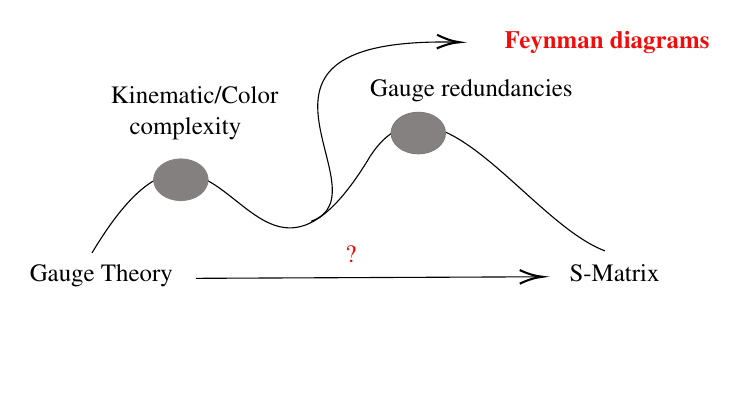
\begin{tikzpicture}[x=0.75pt,y=0.75pt,yscale=-1,xscale=1]
%uncomment if require: \path (0,300); %set diagram left start at 0, and has height of 300

%Curve Lines [id:da3663218891074064] 
\draw    (211.4,171.25) .. controls (275.46,64.25) and (285.26,224.75) .. (345.4,124.75) ;
%Shape: Ellipse [id:dp631421347808582] 
\draw  [color={rgb, 255:red, 134; green, 131; blue, 131 }  ,draw opacity=1 ][fill={rgb, 255:red, 133; green, 128; blue, 128 }  ,fill opacity=1 ] (241.14,136) .. controls (241.14,130.48) and (246.99,126) .. (254.21,126) .. controls (261.43,126) and (267.29,130.48) .. (267.29,136) .. controls (267.29,141.52) and (261.43,146) .. (254.21,146) .. controls (246.99,146) and (241.14,141.52) .. (241.14,136) -- cycle ;
%Curve Lines [id:da0018479507229188785] 
\draw    (345.4,124.75) .. controls (376.12,77.25) and (421.23,156.25) .. (458.49,170.25) ;
%Shape: Ellipse [id:dp37806345751603687] 
\draw  [color={rgb, 255:red, 128; green, 124; blue, 124 }  ,draw opacity=1 ][fill={rgb, 255:red, 133; green, 129; blue, 129 }  ,fill opacity=1 ] (355.53,113.5) .. controls (355.53,107.98) and (361.39,103.5) .. (368.61,103.5) .. controls (375.83,103.5) and (381.68,107.98) .. (381.68,113.5) .. controls (381.68,119.02) and (375.83,123.5) .. (368.61,123.5) .. controls (361.39,123.5) and (355.53,119.02) .. (355.53,113.5) -- cycle ;
%Straight Lines [id:da7438579232631651] 
\draw    (261.4,183.5) -- (426.42,182.76) ;
\draw [shift={(428.42,182.75)}, rotate = 179.74] [color={rgb, 255:red, 0; green, 0; blue, 0 }  ][line width=0.75]    (10.93,-3.29) .. controls (6.95,-1.4) and (3.31,-0.3) .. (0,0) .. controls (3.31,0.3) and (6.95,1.4) .. (10.93,3.29)   ;
%Curve Lines [id:da40606602539843883] 
\draw    (316.97,156) .. controls (355.02,142.32) and (265.25,67.01) .. (386.7,69.7) ;
\draw [shift={(388.54,69.75)}, rotate = 181.61] [color={rgb, 255:red, 0; green, 0; blue, 0 }  ][line width=0.75]    (10.93,-3.29) .. controls (6.95,-1.4) and (3.31,-0.3) .. (0,0) .. controls (3.31,0.3) and (6.95,1.4) .. (10.93,3.29)   ;

% Text Node
\draw (215.9,175.75) node [anchor=north] [inner sep=0.75pt]  [font=\small] [align=left] {{\fontfamily{ptm}\selectfont {\small  Gauge Theory}}\\{\fontfamily{ptm}\selectfont {\small  }}};
% Text Node
\draw (219.25,90) node [anchor=north west][inner sep=0.75pt]  [font=\small] [align=left] {{\small {\fontfamily{ptm}\selectfont Kinematic/Color}}\\{\small {\fontfamily{ptm}\selectfont  \ \ \ complexity}}};
% Text Node
\draw (344.1,86.5) node [anchor=north west][inner sep=0.75pt]  [font=\small] [align=left] {{\fontfamily{ptm}\selectfont {\small Gauge redundancies}}};
% Text Node
\draw (440.24,175.5) node [anchor=north west][inner sep=0.75pt]  [font=\small] [align=left] {{\fontfamily{ptm}\selectfont {\small S-Matrix}}};
% Text Node
\draw (332.23,166.5) node [anchor=north west][inner sep=0.75pt]  [font=\normalsize] [align=left] {{\fontfamily{ptm}\selectfont {\small \textcolor[rgb]{1,0,0}{?}}}};
% Text Node
\draw (408.97,63) node [anchor=north west][inner sep=0.75pt]  [font=\small] [align=left] {{\fontfamily{ptm}\selectfont {\small \textbf{\textcolor[rgb]{0.95,0.05,0.05}{Feynman diagrams}}}}};

\end{tikzpicture}
\end{center}
\vspace{-2.3em}
\pause
\begin{center}
\begin{tabular}{|c|c|c|c|c|c|c|c|}
\hline
$n$ pt. amplitudes & 4 & 5 & 6 & 7 & 8 & 9 & 10 \\
\hline
\# of diagrams      & 4 & 25 & 220 & 2485 & 34300 & 559405 & 10525900 \\
\hline
\end{tabular}
\end{center}
\centering
\textcolor{red}{The number of Feyman diagrams grow quite rapidly!}

\end{frame}

\begin{frame}
\frametitle{Conventional Computation}

    Usually, when we compute the gluon amplitudes by using Feynman diagram, we will obtain something like 
\begin{figure}
  \centering
  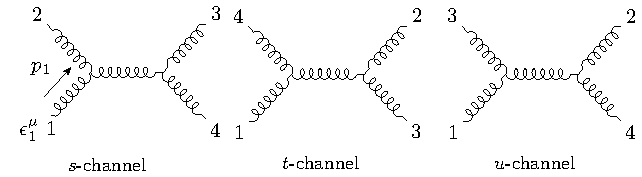
\includegraphics[height=2.5cm]{4ptt2.pdf} \hfill
  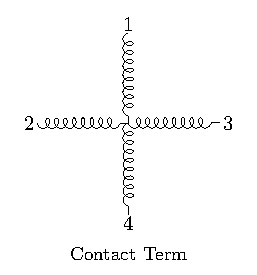
\includegraphics[height=2.8cm]{4ptt2_1.pdf}
\end{figure}


\vspace{-2em}

\begin{flushleft}
$
\begin{aligned}
&\mathcal{M}_s(p_1 p_2 \to p_3 p_4) = - \frac{g_s^2}{s} f^{abe} f^{cde} \\
&\quad \times \Big\{ 
-4\, (\epsilon_1 \cdot \epsilon_3^*) \, (\epsilon_2 \cdot p_1) \, (\epsilon_4^* \cdot p_3) 
+ 2\, (\epsilon_1 \cdot \epsilon_2) \, (\epsilon_3^* \cdot p_1) \, (\epsilon_4^* \cdot p_3) \\
& \quad - 2\, (\epsilon_1 \cdot p_4) \, (\epsilon_2 \cdot p_1) \, (\epsilon_3^* \cdot \epsilon_4^*)
+ (\epsilon_1 \cdot \epsilon_2) \, (p_4 \cdot p_1) \, (\epsilon_3^* \cdot \epsilon_4^*)  + \text{10 terms}\big\}
\end{aligned}
$
\end{flushleft}

\end{frame}

\begin{frame}
If you consider 5point case, it will become worse:
\begin{center}
    \textcolor{red}{$\bigstar$ We have 25 diagrams and nearly 10000 terms!}
\end{center}
\vspace{-2em}
    % 左侧:传统图像

    \textbf{传统费曼图计算:}
    \begin{figure}
        \centering
        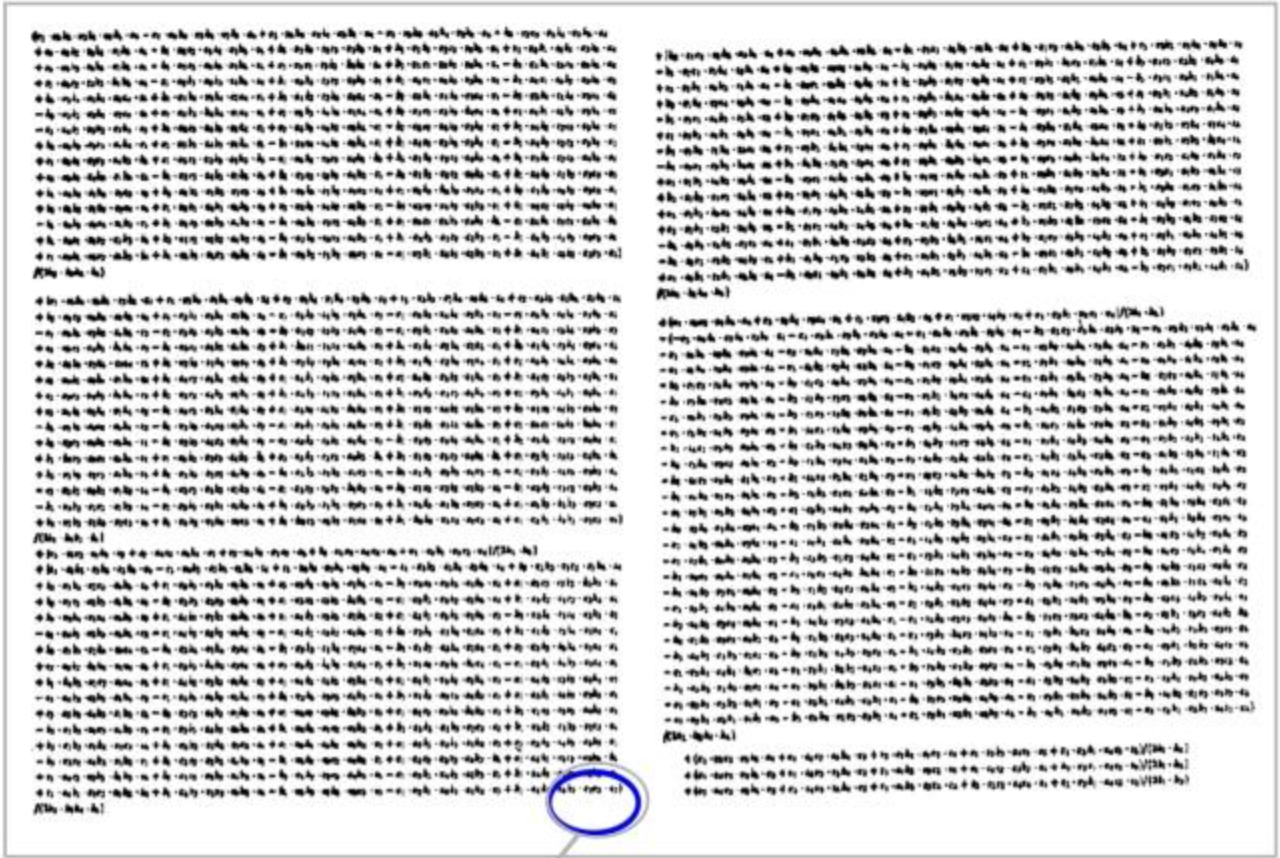
\includegraphics[width=0.5\linewidth]{5pt.png}
    \end{figure}
\vspace{-1.5em}
\pause
\begin{center}
\hspace*{-0.5em}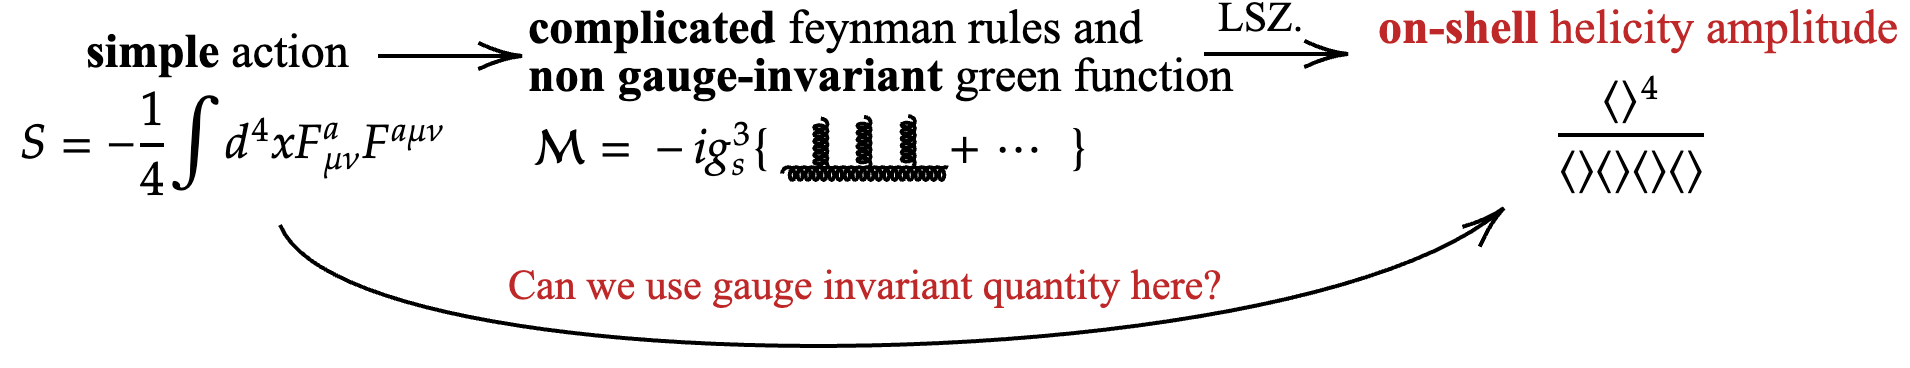
\includegraphics[width=1.05\textwidth]{structure.png}
\end{center}

\end{frame}
\section{Preliminary}
\begin{frame}
\frametitle{Modern Amplitude Method} 
 The answer is On-shell method.
    \begin{center}
        

\tikzset{every picture/.style={line width=0.75pt}} %set default line width to 0.75pt        

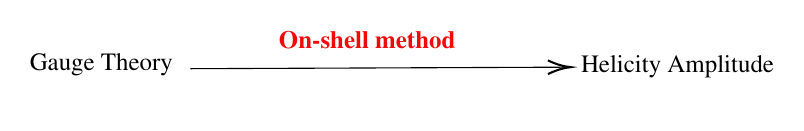
\begin{tikzpicture}[x=0.75pt,y=0.75pt,yscale=-1,xscale=1]
%uncomment if require: \path (0,300); %set diagram left start at 0, and has height of 300

%Straight Lines [id:da5445374886882226] 
\draw    (276.25,137) -- (457.5,136.26) ;
\draw [shift={(459.5,136.25)}, rotate = 179.77] [color={rgb, 255:red, 0; green, 0; blue, 0 }  ][line width=0.75]    (10.93,-3.29) .. controls (6.95,-1.4) and (3.31,-0.3) .. (0,0) .. controls (3.31,0.3) and (6.95,1.4) .. (10.93,3.29)   ;

% Text Node
\draw (233.4,128.25) node [anchor=north] [inner sep=0.75pt]  [font=\small] [align=left] {{\fontfamily{ptm}\selectfont {\small  Gauge Theory}}\\{\fontfamily{ptm}\selectfont {\small  }}};
% Text Node
\draw (463.24,129.5) node [anchor=north west][inner sep=0.75pt]  [font=\small] [align=left] {{\fontfamily{ptm}\selectfont {\small Helicity Amplitude}}};
% Text Node
\draw (317.73,117.5) node [anchor=north west][inner sep=0.75pt]  [font=\normalsize] [align=left] {{\fontfamily{ptm}\selectfont {\small \textbf{\textcolor[rgb]{0.95,0.04,0.04}{On-shell method}}}}};
\end{tikzpicture}
\end{center}
\vspace{-1em}
\pause
$M_5=\!\!\!\!\!\!\underbrace{A_5[12345]}_{\textcolor{red}{\text{Color-ordered Amplitudes}}}\mathrm{Tr}[T^{a_1}T^{a_2}\cdots T^{a_5}]+\text{permutations}$ 

    % 右侧:PT表达式

    \qquad \textbf{Parke–Taylor Formula (MHV amplitudes):}
    \begin{align*}
    A_5[1^+2^+3^+4^+5^+] &= 0 
    \qquad (\!+,-:~\text{\hyperlink{helicity}{helicity};} \\
    A_5[1^-2^+3^+4^+5^+] &= 0 
    \qquad 1,2,\cdots,n:~\text{particle labels}) \\
    \end{align*}
    \vspace{-3em}
    \hypertarget{conv}{}
    \pause
    \begin{gather*}
        {A_5[1^-2^-3^-4^-5^-]=0}\\
        {A_5[1^+2^-3^-4^-5^-]=0}\\
        \textcolor{red}{A_5[1^+2^+3^-4^-5^-]=\frac{[12]^4}{[12][23][34][45][51]}}
    \end{gather*}
\end{frame}

\begin{frame}
    \frametitle{Color-ordering for Yang-Mills}
    Consider the Yang-Mills lagrangian
    \begin{equation*}
        \mathcal{L}=-\frac{1}{2}\mathrm{Tr}(F_{\mu\nu}F^{\mu\nu})
    \end{equation*}
    The 3 point and 4 point vertices include $\tilde{f}^{abc}$ and $\tilde{f}^{abe}\tilde{f}^{cde}+\text{perms}$.

    (With a different convention,$\textrm{Tr}[T^aT^b]=\delta^{ab}$ and $[T^a,T^b]=i\tilde{f}^{abc}T^c$)

    We have 
    \begin{equation*}
        c_s=\tilde{f}^{a_1a_2b}\tilde{f}^{ba_3a_4},\quad c_t=\tilde{f}^{a_4a_1b}\tilde{f}^{ba_2a_3},\quad c_u=\tilde{f}^{a_1a_3b}\tilde{f}^{ba_2a_4}
    \end{equation*}
    and the color factor can be rewritten by the trace of product of generators
    \begin{equation*}
        i\tilde{f}^{abc}=\mathrm{Tr}([T^a,T^b]T^c),
    \end{equation*}
    Moreover, in $SU(N)$, we have a Fierz identity
    \begin{equation}
        \sum_{a}T^a_{ij}T^a_{kl}=\delta_{il}\delta_{kj}-\frac{1}{N}\delta_{ij}\delta_{kl}.
    \end{equation}
\end{frame}
    
\begin{frame}
    This identity is easier understood as matrix form like 
    \begin{align*}
    \mathrm{Tr}\{T^aA\}\mathrm{Tr}\{T^aB\}=\mathrm{Tr}\{AB\}-\frac{1}{N}\mathrm{Tr}\{A\}\mathrm{Tr}\{B\},\\
    \mathrm{Tr}\{AT^aBT^a\}=\mathrm{Tr}\{A\}\mathrm{Tr}\{B\}-\frac{1}{N}\mathrm{Tr}\{AB\}.
    \end{align*}
    So, the 4 gluon s-channel gives us
    \begin{align*}
        \tilde{f}^{a_1a_2b}\tilde{f}^{ba_3a_4}=\mathrm{Tr}(T^{a_1}T^{a_2}T^{a_3}T^{a_4})-\mathrm{Tr}(T^{a_2}T^{a_1}T^{a_3}T^{a_4})\\
        -\mathrm{Tr}(T^{a_1}T^{a_2}T^{a_4}T^{a_3})+\mathrm{Tr}(T^{a_2}T^{a_1}T^{a_4}T^{a_3}).
    \end{align*}
    Therefore, the full 4-point amplitude can be rewritten like
    \begin{equation*}
        \mathcal{A}_{4,\text{tree}}=g^2(A_4[1234]\mathrm{Tr}(T^{a_1}T^{a_2}T^{a_3}T^{a_4})+\text{perms of } (234) )
    \end{equation*}
    here the subamplitudes $A_4[1234],A_4[1243]$, etc. are called \textbf{color-ordered ampltitudes}. This concept can be easily generalized to tree-level n-point case
    \begin{equation*}
        \textcolor{red}{\mathcal{A}_{n,\text{tree}}=g^{n-2}\sum_{\sigma}A_n[1,\sigma(2,3\cdots n)]\mathrm{Tr}(T^{a_1}T^{\sigma(a_2\cdots}T^{a_n)})}
    \end{equation*}
\end{frame}

\begin{frame}
    \frametitle{The Power of BCFW Recursion Relation}
    %First, I will show the most important part in this report.
    \begin{block}{BCFW recursion relation}
        \begin{equation*}
            A_n=\sum_{\text{diagrams}\,I}\hat{A}_L(z_I)\frac{1}{P_I^2}\hat{A}_R(z_I)=\sum_{\text{diagrams}\,I}\raisebox{-1.3em}{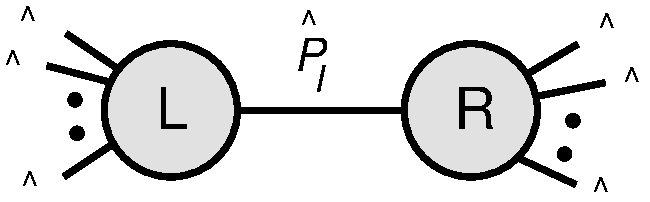
\includegraphics[height=3em]{recrel1.pdf}}
        \end{equation*}
    \end{block}
\vspace*{1em}
\pause
\tikzset{every picture/.style={line width=0.75pt}} %set default line width to 0.75pt        

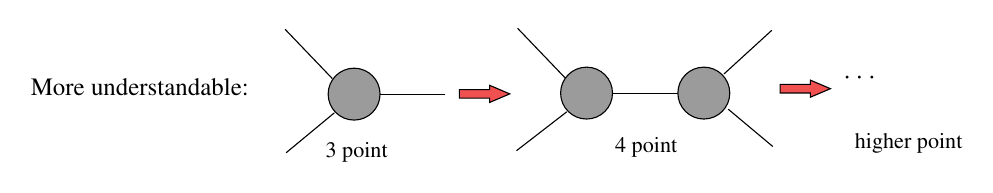
\begin{tikzpicture}[x=0.75pt,y=0.75pt,yscale=-1,xscale=1]
%uncomment if require: \path (0,300); %set diagram left start at 0, and has height of 300

%Shape: Circle [id:dp714548377068662] 
\draw  [fill={rgb, 255:red, 155; green, 155; blue, 155 }  ,fill opacity=1 ] (226.5,142.5) .. controls (226.5,135.6) and (232.1,130) .. (239,130) .. controls (245.9,130) and (251.5,135.6) .. (251.5,142.5) .. controls (251.5,149.4) and (245.9,155) .. (239,155) .. controls (232.1,155) and (226.5,149.4) .. (226.5,142.5) -- cycle ;
%Straight Lines [id:da2774899580018806] 
\draw    (205.75,111.25) -- (228.5,135) ;
%Straight Lines [id:da9722977180083648] 
\draw    (206.25,170.75) -- (229.5,151.5) ;
%Straight Lines [id:da6995788762725553] 
\draw    (283,142.5) -- (251.5,142.5) ;
%Shape: Circle [id:dp5472781658369114] 
\draw  [fill={rgb, 255:red, 155; green, 155; blue, 155 }  ,fill opacity=1 ] (338.5,142) .. controls (338.5,135.1) and (344.1,129.5) .. (351,129.5) .. controls (357.9,129.5) and (363.5,135.1) .. (363.5,142) .. controls (363.5,148.9) and (357.9,154.5) .. (351,154.5) .. controls (344.1,154.5) and (338.5,148.9) .. (338.5,142) -- cycle ;
%Straight Lines [id:da00014298672423462833] 
\draw    (317.75,110.75) -- (340.5,134.5) ;
%Straight Lines [id:da9890078833503395] 
\draw    (317.25,169.75) -- (341.5,151) ;
%Straight Lines [id:da6144558640267263] 
\draw    (395,142) -- (363.5,142) ;
%Right Arrow [id:dp2461212615941556] 
\draw  [fill={rgb, 255:red, 241; green, 80; blue, 80 }  ,fill opacity=1 ] (289.75,140.31) -- (304.3,140.31) -- (304.3,138.25) -- (314,142.38) -- (304.3,146.5) -- (304.3,144.44) -- (289.75,144.44) -- cycle ;
%Shape: Circle [id:dp17520461351076555] 
\draw  [fill={rgb, 255:red, 155; green, 155; blue, 155 }  ,fill opacity=1 ] (395,142) .. controls (395,135.1) and (400.6,129.5) .. (407.5,129.5) .. controls (414.4,129.5) and (420,135.1) .. (420,142) .. controls (420,148.9) and (414.4,154.5) .. (407.5,154.5) .. controls (400.6,154.5) and (395,148.9) .. (395,142) -- cycle ;
%Straight Lines [id:da6771243917531791] 
\draw    (417.25,132.75) -- (440.25,111.75) ;
%Straight Lines [id:da9753272478311303] 
\draw    (419.25,149.75) -- (440.75,167.75) ;
%Right Arrow [id:dp8085176402619464] 
\draw  [fill={rgb, 255:red, 241; green, 80; blue, 80 }  ,fill opacity=1 ] (444.25,137.81) -- (458.8,137.81) -- (458.8,135.75) -- (468.5,139.88) -- (458.8,144) -- (458.8,141.94) -- (444.25,141.94) -- cycle ;

% Text Node
\draw (82,133.5) node [anchor=north west][inner sep=0.75pt]   [align=left] {{\fontfamily{ptm}\selectfont {\small More understandable:}}};
% Text Node
\draw (473.5,130.9) node [anchor=north west][inner sep=0.75pt]    {$\cdots $};
% Text Node
\draw (224,164.5) node [anchor=north west][inner sep=0.75pt]   [align=left] {{\fontfamily{ptm}\selectfont {\footnotesize 3 point}}};
% Text Node
\draw (363.5,162) node [anchor=north west][inner sep=0.75pt]   [align=left] {{\fontfamily{ptm}\selectfont {\footnotesize 4 point}}};
% Text Node
\draw (479,160) node [anchor=north west][inner sep=0.75pt]   [align=left] {{\fontfamily{ptm}\selectfont {\footnotesize higher point}}};

\end{tikzpicture}

\vspace{1em}

\textcolor{red}{$\bigstar $ ~ From lower point on-shell amp. to higher point on-shell amp.!!}

\end{frame}

\begin{frame}
    \frametitle{Momentum Shift in BCFW}
    \textbf{What did BCFW do to make the shift?}

    Here we consider the case in which all particles are massless, $p_i^2 = 0$ for all $i = 1, 2, \dotsc, n$. We choose two momentum to be shifted oppositely 
    \begin{equation*}
        p_i\rightarrow\hat{p}_i(z)\equiv p_i-zk,\qquad p_j\rightarrow\hat{p}_j(z)\equiv p_j+zk
    \end{equation*}
    satisfying 
    \begin{equation*}
        k^2=0,\qquad p_i\cdot k=0,\qquad p_j\cdot k=0
    \end{equation*}

\begin{figure}
    \centering
    \begin{minipage}{0.45\textwidth}
        \tikzset{every picture/.style={line width=0.75pt}} %set default line width to 0.75pt        

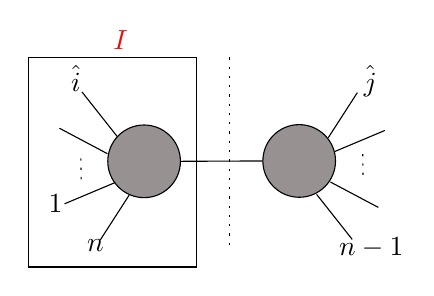
\begin{tikzpicture}[scale=0.7,x=0.75pt,y=0.75pt,yscale=-1,xscale=1]
%uncomment if require: \path (0,300); %set diagram left start at 0, and has height of 300

%Shape: Circle [id:dp47058391497271046] 
\draw  [fill={rgb, 255:red, 151; green, 145; blue, 145 }  ,fill opacity=1 ] (266.75,126) .. controls (266.75,112.19) and (277.94,101) .. (291.75,101) .. controls (305.56,101) and (316.75,112.19) .. (316.75,126) .. controls (316.75,139.81) and (305.56,151) .. (291.75,151) .. controls (277.94,151) and (266.75,139.81) .. (266.75,126) -- cycle ;
%Straight Lines [id:da8759716500759761] 
\draw    (249,78.25) -- (273.5,109.25) ;
%Straight Lines [id:da2121821831988906] 
\draw    (233.5,103.25) -- (266.5,120.75) ;
%Straight Lines [id:da6378763431676462] 
\draw  [dash pattern={on 0.84pt off 2.51pt}]  (350.75,54.38) -- (350.75,126.25) -- (350.75,187.63) ;
%Straight Lines [id:da7508961107891289] 
\draw  [dash pattern={on 0.84pt off 2.51pt}]  (248.25,124) -- (248.5,142.25) ;
%Straight Lines [id:da06317949320750826] 
\draw    (237,155.25) -- (271.5,140.75) ;
%Straight Lines [id:da403008866951158] 
\draw    (261.5,180.25) -- (281.5,149.25) ;
%Straight Lines [id:da8334043101335312] 
\draw    (423,119.25) -- (457.5,104.75) ;
%Straight Lines [id:da03451573841415356] 
\draw    (418.5,109.75) -- (438.5,78.75) ;
%Straight Lines [id:da025418352459996796] 
\draw    (420,140.25) -- (453,157.75) ;
%Straight Lines [id:da22879254297825424] 
\draw  [dash pattern={on 0.84pt off 2.51pt}]  (442.25,121) -- (442.5,139.25) ;
%Straight Lines [id:da2355772127149045] 
\draw    (410.5,148.75) -- (435,179.75) ;
%Shape: Rectangle [id:dp6752662310096104] 
\draw   (328,54.25) -- (328,198.75) -- (212,198.75) -- (212,54.25) -- cycle ;
%Straight Lines [id:da4580921639862495] 
\draw    (316.75,126) -- (373.5,125.75) ;
%Shape: Circle [id:dp8699671429684472] 
\draw  [fill={rgb, 255:red, 151; green, 145; blue, 145 }  ,fill opacity=1 ] (373.5,125.75) .. controls (373.5,111.94) and (384.69,100.75) .. (398.5,100.75) .. controls (412.31,100.75) and (423.5,111.94) .. (423.5,125.75) .. controls (423.5,139.56) and (412.31,150.75) .. (398.5,150.75) .. controls (384.69,150.75) and (373.5,139.56) .. (373.5,125.75) -- cycle ;

% Text Node
\draw (239.75,58.4) node [anchor=north west][inner sep=0.75pt]    {$\hat{i}$};
% Text Node
\draw (447.47,58.4) node [anchor=north] [inner sep=0.75pt]    {$\hat{j}$};
% Text Node
\draw (250.75,177.9) node [anchor=north west][inner sep=0.75pt]    {$n$};
% Text Node
\draw (224.25,147.4) node [anchor=north west][inner sep=0.75pt]    {$1$};
% Text Node
\draw (424.25,176.9) node [anchor=north west][inner sep=0.75pt]    {$n-1$};
% Text Node
\draw (268.75,34.4) node [anchor=north west][inner sep=0.75pt]  [color={rgb, 255:red, 241; green, 12; blue, 12 }  ,opacity=1 ]  {$I$};


\end{tikzpicture}
    \end{minipage}
    \hspace{1em}
    \begin{minipage}{0.45\textwidth}
        For a non-trival subset of generic momenta $\{p_i\}_{i\in I}$
    \begin{equation*}
        \hat{P}_I^2=P_I^2 -2zP_I\cdot k=-\frac{P_I^2}{z_I}(z-z_I) 
    \end{equation*}

    with $\textcolor{red}{\quad z_I=\frac{P_I^2}{2P_I\cdot k}}$.  
    \end{minipage}
\end{figure} 
\end{frame}

\begin{frame}
    
    \textbf{Brief explaination}: We choose two momentum to be shifted oppositely 
    \begin{equation*}
        p_i\rightarrow\hat{p}_i(z)\equiv p_i-zk,\qquad p_j\rightarrow\hat{p}_j(z)\equiv p_j+zk
    \end{equation*}
    satisfying 
    \begin{equation*}
        k^2=0,\qquad p_i\cdot k=0,\qquad p_j\cdot k=0
    \end{equation*}
    
    We consider amplitude $A_n$ in terms of shifted momentum $\hat{p}_i^\mu$ instead of original real momentum. 
    \begin{equation*}
        A_n \longrightarrow \hat{A}_n(z)
    \end{equation*}
    \pause
    If we consider the meromorphic function $\frac{\hat{A}_n(z)}{z}$ in the complex plane.
    From Cauchy Theorem, we can ontain
    \begin{equation*}
        A_n=-\sum_{z_I}\textrm{Res}|_{z=z_I}\frac{\hat{A}_n(z)}{z}+B_n,
    \end{equation*}
    where $B_n$ is the residue of the pole at $z=\infty$, called boundary term.
\end{frame}

\begin{frame}
    From Cauchy Theorem, we can ontain
    \begin{equation*}
        A_n=-\sum_{z_I}\textrm{Res}|_{z=z_I}\frac{\hat{A}_n(z)}{z}+B_n,
    \end{equation*}
    where $B_n$ is the residue of the pole at $z=\infty$, called boundary term.
    \vspace{-1em}
    \begin{figure}[htbp]
        \centering
        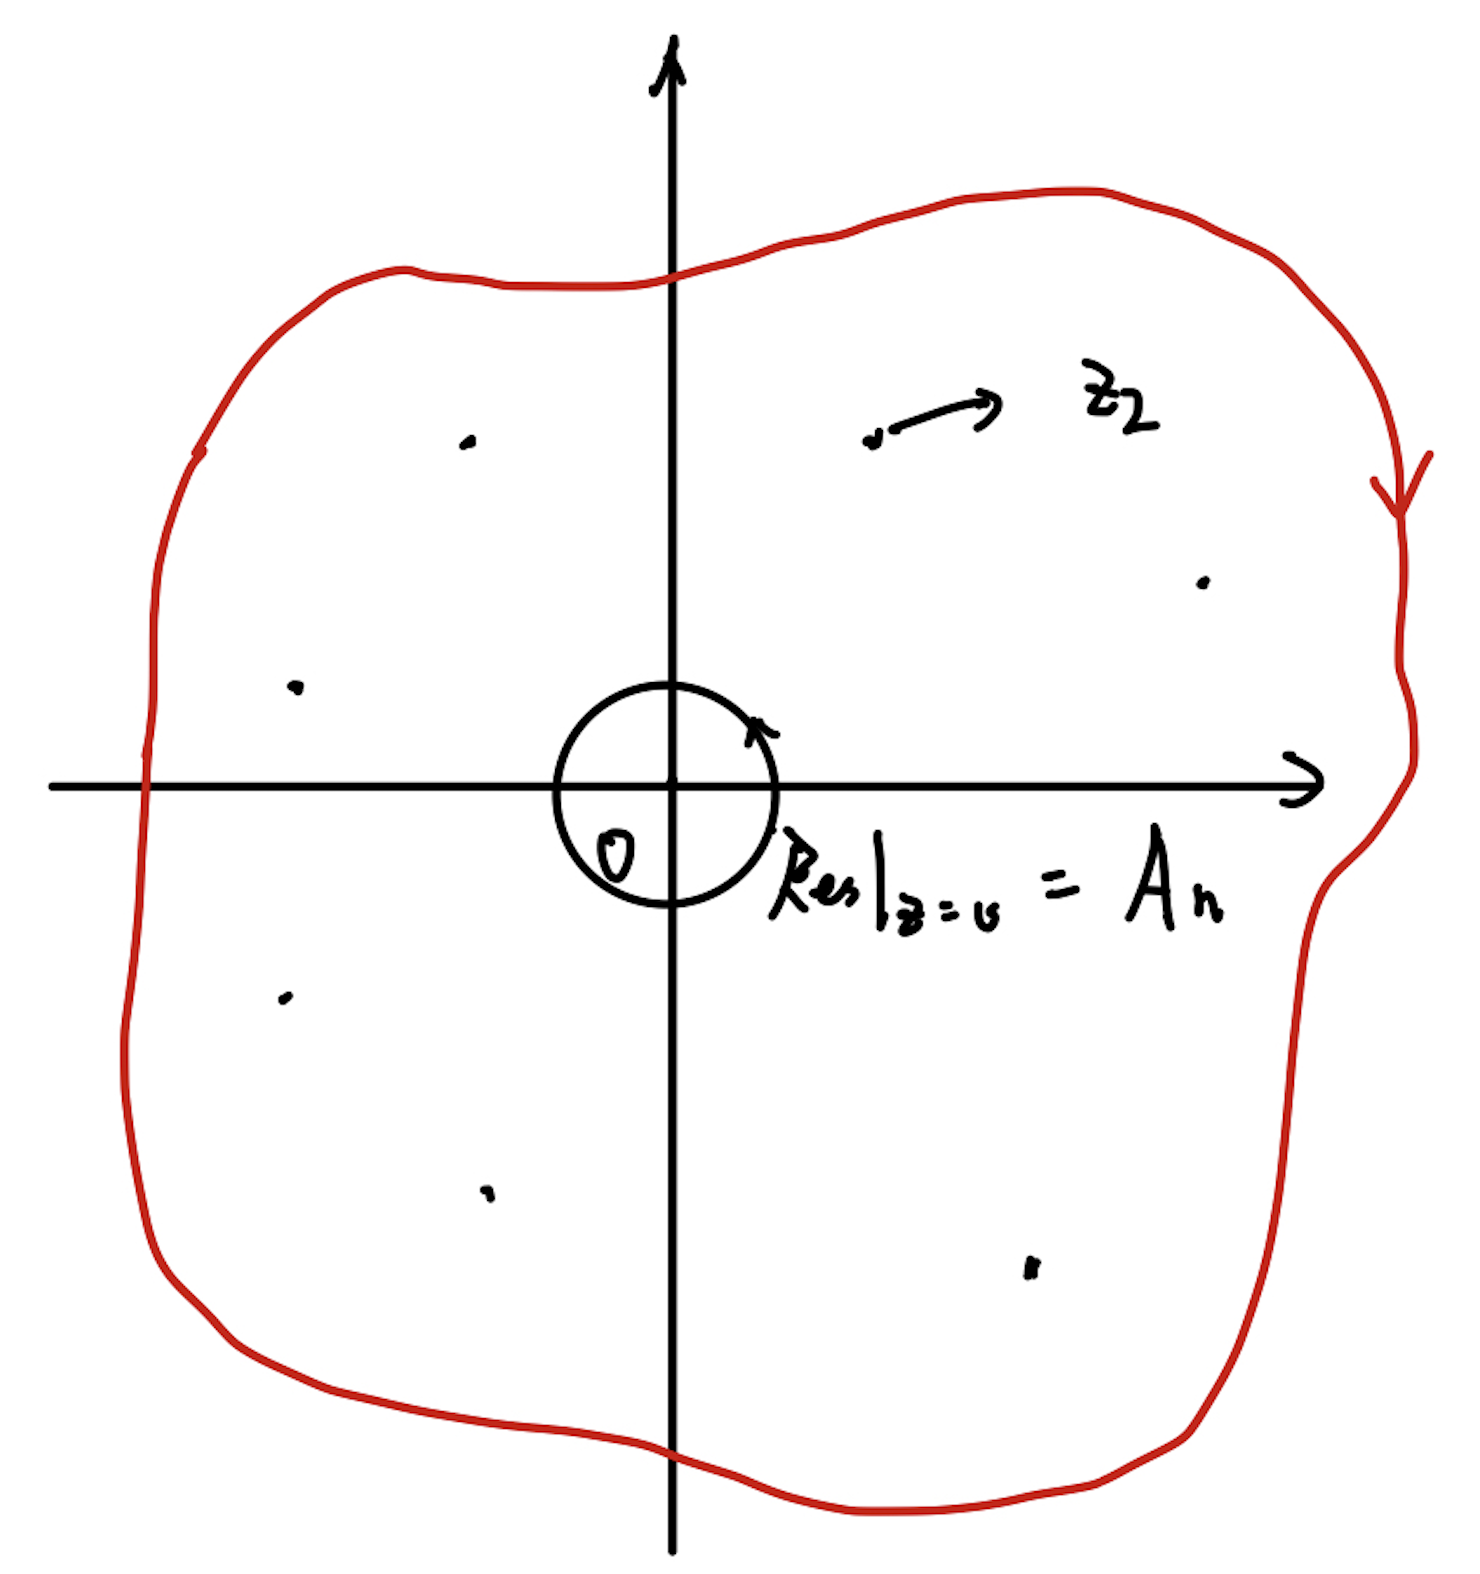
\includegraphics[width=0.3\textwidth]{CT.png}
    \end{figure}
    \vspace{-1.5em}
    %Then, at a $z_I$ pole, the propagator $\hat{P}_I^2$ goes to on-shell. In that limit, the shifted amplitude
    %\textcolor{red}{factorizes} into to on-shell parts (Unitarity)
    \begin{equation*}
        \hat{A}_n(z)\quad \xrightarrow{z\,\text{near}\,z_I} \quad \hat{A}_L(z_I)\frac{1}{\hat{P}_I^2}\hat{A}_R(z_I)= - \frac{z_I}{z-z_I}\hat{A}_L(z_I)\frac{1}{P_I^2}\hat{A}_R(z_I)
    \end{equation*}
    This makes it easy to evaluate the residue at $z=z_I$
    \begin{equation*}
        -\mathrm{Res}|_{z=z_I}\frac{\hat{A}_n(z)}{z}=\frac{(z-z_I)z_I}{z(z-z_I)}\hat{A}_L(z_I)\frac{1}{P_I^2}\hat{A}_R(z_I)|_{z=z_I}=\hat{A}_L(z_I)\frac{1}{P_I^2}\hat{A}_R(z_I)
    \end{equation*}
\end{frame}

\begin{frame}
    \frametitle{Large z behavior}
    In the BCFW formula, the boundary term $B_n$ affects a lot
    \begin{equation*}
        A_n=-\sum_{z_I}\mathrm{Res}|_{z=z_I}\frac{\hat{A}_n(z)}{z}+B_n,
    \end{equation*}
    In most applications. one assumes or much better, proves $B_n=0$. This is often justified by declaring a stronger condition
    \begin{equation*}
        \textcolor{red}{\hat{A}_n(z)\rightarrow 0 \quad \text{for} \quad z\rightarrow \infty} 
    \end{equation*}
    Here I show the large z behavior for gluon scattering 
    \begin{center}
        \begin{tabular}{lrc}
            \toprule
            $[i\, \textbackslash \, j\rangle $ & $+$ & $-$ \\
            \midrule
            $+$ & $1/z$ & $z^3$ \\
            $-$ & $1/z$ & $1/z$ \\
            \bottomrule
          \end{tabular}
    \end{center}
    proved by using background field expansion ~\textcolor{green}{(N.~Arkani-Hamed and J.~Kaplan,
%``On Tree Amplitudes in Gauge Theory and Gravity,''
[arXiv:0801.2385 [hep-th]].)}
\end{frame}

\begin{frame}
\frametitle{Little group scaling}
    \begin{itemize}
        \item $\textbf{\text{Massless Case}}$\\
    \begin{equation*}
        p_\mu \sigma^\mu=p_{\alpha\dot{\alpha}}=\lambda_\alpha \tilde{\lambda}_{\dot{\alpha}}=\aket{\lambda}[\lambda|
    \end{equation*}
    There is an ambiguity for the definition, the momentum is invariant under the following redefinition
    \begin{equation*}
        \lambda \rightarrow t^{-1}\lambda, \qquad \tilde{\lambda}\rightarrow t\tilde{\lambda}, \qquad t\in\mathbb{C} 
    \end{equation*}
    same for
    \begin{equation*}
        \aket{\lambda}\rightarrow t^{-1}\aket{\lambda}, \qquad \sket{\lambda}\rightarrow t\sket{\lambda}
    \end{equation*}
    The scattering amplitudes should transform \textcolor{red}{covariantly} under little group scaling:
    \begin{equation*}
        \color{red} \mathcal{A}_n(\{\aket{1},\sket{1},h_1\},\ldots\{t_i^{-1}\aket{i},t_i\sket{i},h_i\},\ldots )=t_i^{2h_i}\mathcal{A}_n
    \end{equation*}
    \end{itemize}
\vspace{-2em}
    \begin{itemize}
    \item \textbf{Massive Case}\\
    It can also be handled in terms of spinor-helicity variable, see also 	arXiv:1709.04891 [hep-th] (Nima Arkani-Hamed, Tzu-Chen Huang, Yu-tin Huang).
    \end{itemize}
\end{frame}


\begin{frame}
    \frametitle{ On-shell 3-point can be completely determined}
    \textbf{Another necessarity to introduce complex momentum}
    If the momentum is complexed, we have 
    \begin{equation*}
        \avg{12}\neq[21]^*
    \end{equation*}
    Then we can obtain
    \begin{equation*}
        \aket{1}\propto \aket{2}\propto \aket{3} \qquad or \qquad \sket{1}\propto \sket{2}\propto \sket{3}
    \end{equation*}
    It means that 3-point amplitude depends only on angle brackets or squar brackets. Here I choose the first case to give an example
    \begin{equation*}
        A_3(1^{h_1},2^{h_2},3^{h_3})=c\avg{12}^{x_{12}}\avg{13}^{x_{13}}\avg{23}^{x_{23}},
    \end{equation*}
    Little group scaling tells us that
    \begin{equation*}
        t_1^{2h_1} A_3(1^{h_1},2^{h_2},3^{h_3})=ct_1^{-x_{12}}t_1^{-x_{13}}\avg{12}^{x_{12}}\avg{13}^{x_{13}}\avg{23}^{x_{23}}.
    \end{equation*}
    We can obtain
    \begin{equation*}
        2h_1=-x_{12}-x_{13}
    \end{equation*}
    Similarly, we can also obtain
    \begin{equation*}
        2h_2=-x_{12}-x_{23},\qquad 2h_3=-x_{13}-x_{23}.
    \end{equation*}
\end{frame}

\begin{frame}
    Then all index can be solved from this system of equations, so that
    \[
    \boxed{
    \begin{aligned}
        A_3^{h_1h_2h_3} &= c\avg{12}^{h_3-h_1-h_2}\avg{31}^{h_2-h_1-h_3}\avg{23}^{h_1-h_2-h_3}
        \quad & h_1+h_2+h_3 < 0 \\[0.5em]
        A_3^{h_1h_2h_3} &= c' [12]^{h_1+h_2-h_3}[23]^{h_2+h_3-h_1}[31]^{h_3+h_1-h_2}
        \quad & h_1+h_2+h_3 > 0
    \end{aligned}
        }
    \]

    \textbf{\textcolor{red}{$\star$\,All massless on-shell 3-point ampltides are completely determined by little group scaling!}}
    
    \textbf{Example}: 3-gluon amplitude\\
    \begin{equation*}
        A_3(g_1^-,g_2^-,g_3^+)=g\frac{\avg{12}^3}{\avg{23}\!\avg{31}}
    \end{equation*}
    There's another possibility 
    \begin{equation*}
        A_3(g_1^-,g_2^-,g_3^+)=g'\frac{[13][23]}{[12]^3}
    \end{equation*}
    but actually it comes from the \textcolor{red}{non-local} interaction $g'AA\frac{\partial}{\square}A$, so we discard it.
\end{frame}

\begin{frame}{From Review to Applications}

\begin{columns}[T]
  % 左列:当前已完成
  \begin{column}{0.48\textwidth}
    \begin{block}{\centering\large \textbf{So far: Foundations}}
      \begin{itemize}[left=1em]
        \item Reviewed the structure of \textbf{BCFW recursion relation}
        \item Applied to:
          \begin{itemize}[left=0.1em]
            \item \textbf{Pure Yang-Mills} theory
            \item Tree-level MHV amplitudes
            \item Color-ordered partial amplitudes
          \end{itemize}
      \end{itemize}
    \end{block}
  \end{column}
\pause
  % 右列:研究目标
  \begin{column}{0.48\textwidth}
    \begin{block}{\centering\large \textbf{Next: Realistic Models}}
      \begin{itemize}[left=1em]
        \item Move beyond massless gauge theory
        \item Consider:
          \begin{itemize}[left=0.1em]
            \item \textbf{(De)constructed gauge theories}
          \end{itemize}
        \item Key questions:
          \begin{itemize}[left=0.1em]
            \item Can BCFW still apply?
            \item What new structures emerge?
          \end{itemize}
      \end{itemize}
    \end{block}
  \end{column}
\end{columns}

\end{frame}

\section{Model and Computation}

\begin{frame}{Introduction of (De)Constructed gauge theory}
\vspace{1em}
\begin{columns}[c]
    \column{0.43\textwidth}
    \centering
    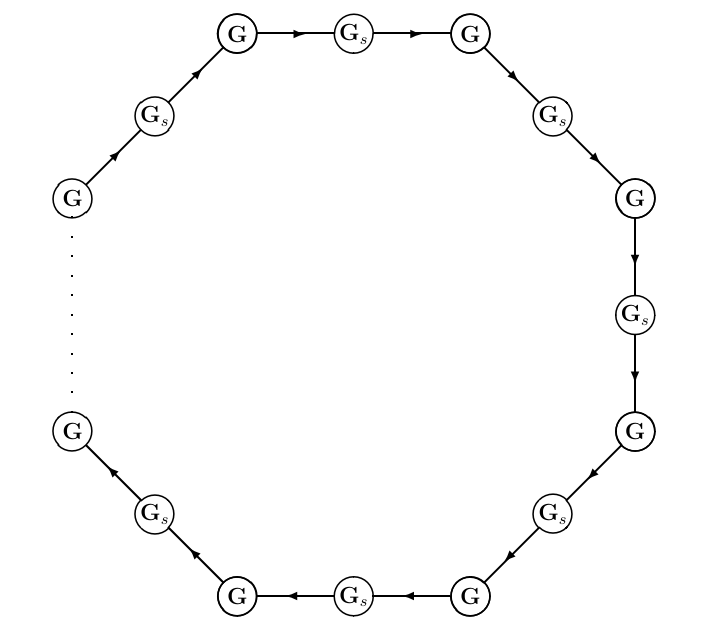
\includegraphics[width=100pt]{Moose.png}

    \column{0.14\textwidth}
    \centering
    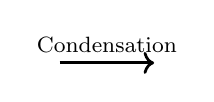
\begin{tikzpicture}[scale=0.8]
        \draw[->, line width=1pt] (0,0) -- (1.5,0)
            node[midway, above] {\footnotesize Condensation}; % ← 加文字
    \end{tikzpicture}

    \column{0.43\textwidth}
    \centering
    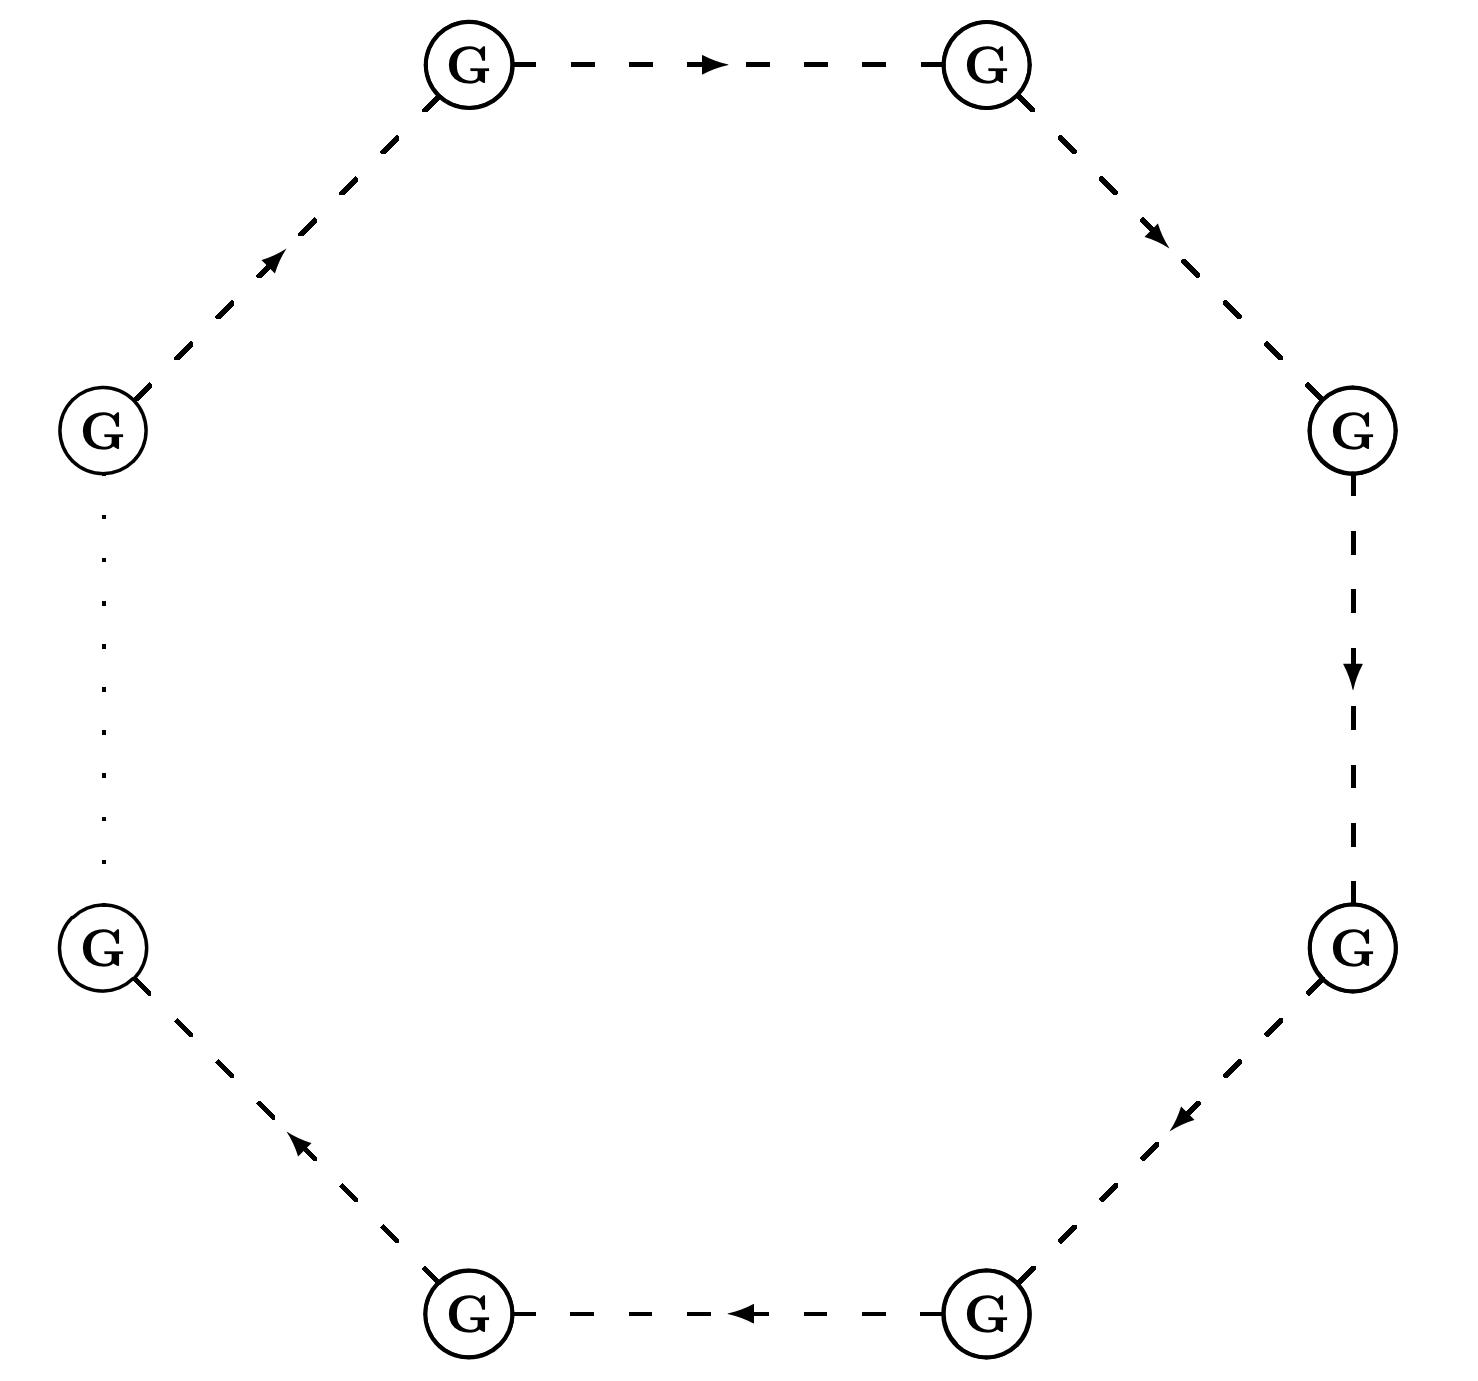
\includegraphics[width=100pt]{Moosed.jpeg}
\end{columns}


\pause
\raggedright
The Lagrangian can be written like
\begin{equation*}
    \mathcal{L} = -\sum_{i=1}^{N} \frac{1}{2} \mathrm{Tr}(F_i^2)
    + \sum_{i=1}^{N} \mathrm{Tr}\left[(D_\mu \Phi_i)^\dagger (D^\mu \Phi_i)\right],
\end{equation*}
here $F_i$ refers to the $i$th gauge field strength. The scalar field $\Phi_i$ transforms under the \textcolor{red}{bi-fundamental} representation, and the covariant derivative equals to
\begin{equation*}
    D_\mu \Phi_i = \partial_\mu \Phi_i - i g_i A_{i\mu} \Phi_i + i g_{i+1} \Phi_i A_{i+1\mu}.
\end{equation*}

\end{frame}

\begin{frame}
    It has been proposed that this model actually discretized \textcolor{red}{a five-dimension gauge theory} with gauge group $SU(m)$, where 
    only the fifth dimension are latticed. So it is an effective theory for 5d gauge theory.
     \vspace{1em} % 图与文字之间的间距
    \begin{center}
    \begin{minipage}{0.45\textwidth}
        \centering
        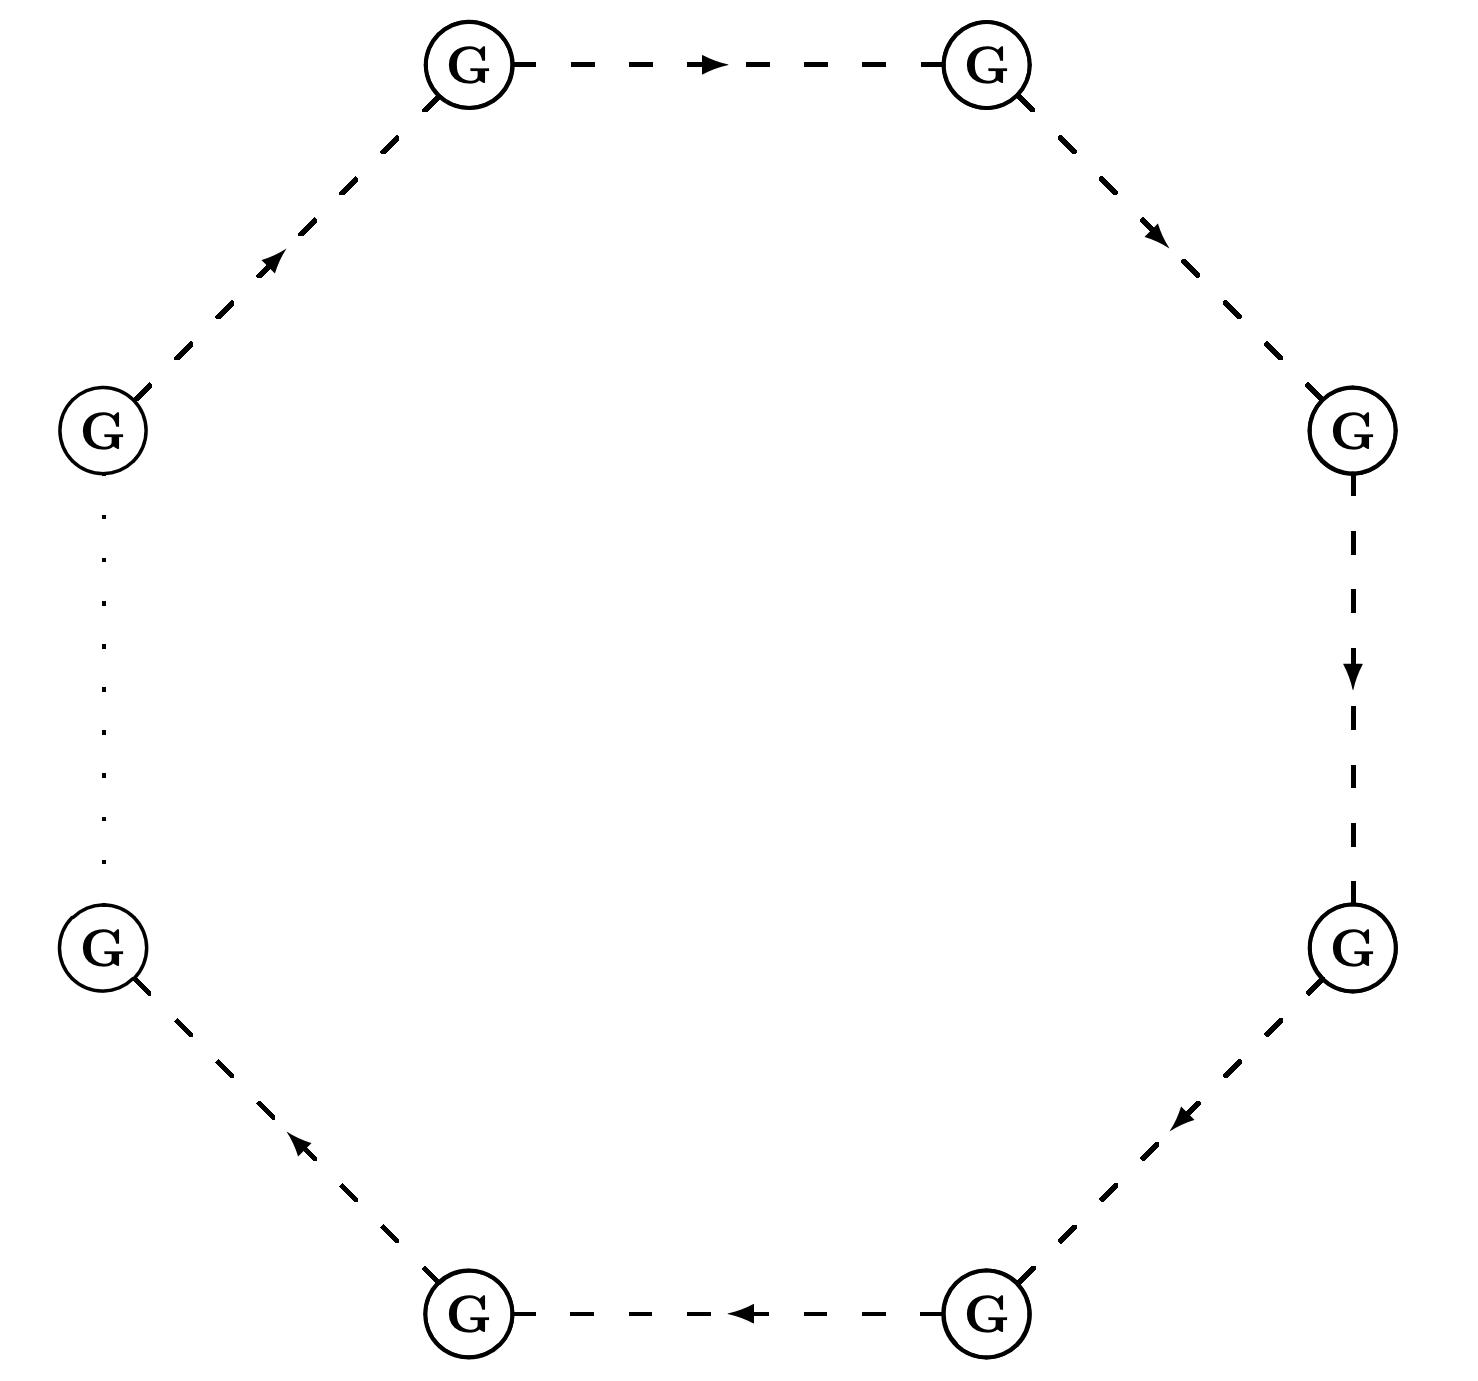
\includegraphics[width=0.6\linewidth]{Moosed.jpeg} % ← 替换为你的图片文件名
        \par\vspace{0.5em}
    \end{minipage}
    \hspace{0.05\textwidth}
    \begin{minipage}{0.45\textwidth}
        \centering
        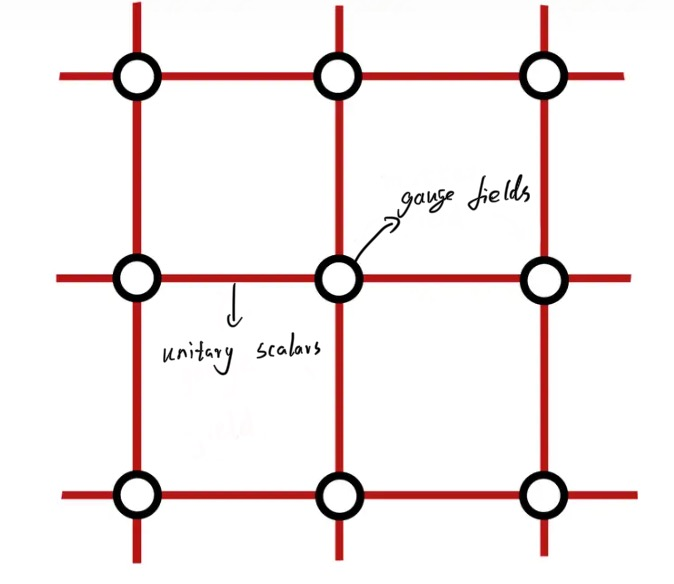
\includegraphics[width=0.6\linewidth]{Lattice.jpg} % ← 替换为你的图片文件名
        \par\vspace{0.5em}
    \end{minipage}
    \end{center}
    \pause
    After higgsing the scalar field, we can obtain a spectrum
    \begin{equation*}
        M_k^2=4g^2f_s^2\sin^2\left(\frac{\pi k}{N}\right)
    \end{equation*}
    This is precisely the \textcolor{red}{Kaluza-Klein} spectrum under $S^1$ compactification. 
\end{frame}

\begin{frame}
    \frametitle{Amplitudes from BCFW}
    \begin{figure}
        \centering
        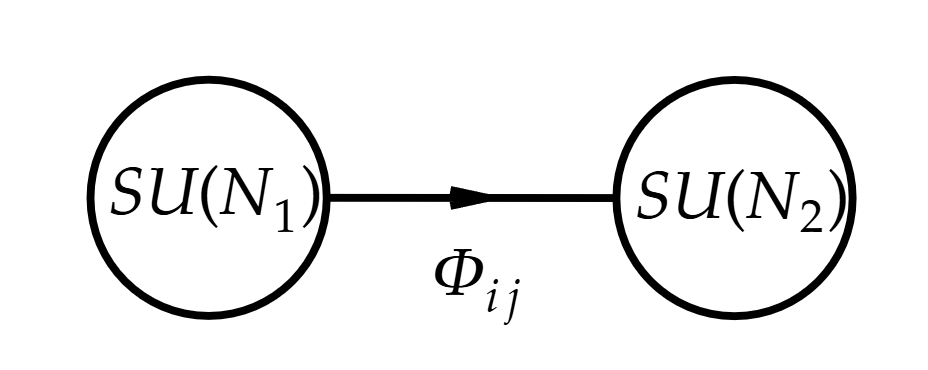
\includegraphics[width=0.5\textwidth]{2-site.png}
    \end{figure}
    \vspace{-1em}
    \begin{equation*}
        \mathcal{L}=-\frac{1}{2}\mathrm{Tr}(F_1)^2-\frac{1}{2}\mathrm{Tr}(F_2)^2+\mathrm{Tr}[(D_\mu\Phi)^\dagger(D^\mu\Phi)],
    \end{equation*}
    From the Lagrangian, we have known that there are only two kinds of 3 point amplitude ($+,-:$ helicity\qquad $\Phi,\Phi^\dagger: \text{charge of scalar}$)
    \begin{gather*}
        A[1^\Phi2^{\Phi^\dagger}3^+]=\frac{[23][31]}{[12]},\qquad A[1^\Phi2^{\Phi^\dagger}3^-]=\frac{\avg{23}\!\avg{31}}{\avg{12}}\\
        A[3^+4^+5^-]=\frac{[34]^3}{[45][53]},\qquad A[3^-4^-5^+]=\frac{\avg{34}^3}{\avg{45}\!\avg{53}}
    \end{gather*}
    By using the 3 point building block, we can construct 4 point colorordered amplitudes from BCFW recursion relation.
\end{frame}
\begin{frame}
    \frametitle{Gauge boson sector}
    \begin{itemize}
        \item n$ V_1$ or n$V_2$\\
        This part is completely the same as the pure gluon amplitude, so we can directly borrow the
        existing results.
        \begin{equation*}
            \boxed{\text{Parke - Talyor Formula}:\quad A[\cdots i^-\cdots j^-\cdots]=\frac{\avg{ij}^4}{\avg{12}\!\avg{23}\cdots\avg{n1}}}
        \end{equation*}
        \textcolor{red}{Notice that this formula only applies to MHV amplitudes, although the NMHV can be completely solved.}
    \end{itemize}
\end{frame}

\begin{frame}
    \frametitle{SQCD like sector}
    The color factor in this sector looks like
    \begin{equation*}
        (T^{a_1}T^{a_2}\cdots T^{a_n})_{ij}
    \end{equation*}
    so we we need to notice is just the order of gauge boson.

    The amplitudes can be computed like 
    \begin{itemize}
        \item $\Phi^\dagger V_1V_1\Phi$
        \begin{align*}
            A[1^\Phi2^{\Phi^\dagger}3^+4^-]=(-1)\frac{\avg{14}^2\avg{24}^2}{\mdavg{12}{23}\!\mdavg{34}{41}}\quad (\textcolor{red}{\text{Parke -Talyor like Formula}})
        \end{align*}
        \item $\Phi^\dagger V_1V_1V_1\Phi$
            \begin{equation*}
                A[1^\Phi2^{\Phi^\dagger}3^+4^+5^-]=\frac{\avg{15}^2\!\avg{25}^2}{\mdavg{12}{23}\!\mdavg{34}{45}\!\avg{51}}
            \end{equation*}
    \end{itemize}
\end{frame}

\begin{frame}
    \begin{itemize}
        \item $\Phi^\dagger (nV_1)\Phi$
            \begin{equation*}
                A[1^\Phi2^{\Phi^\dagger}\cdots(n+2)^-]=(-1)^{n+1}\frac{\avg{1,n+2}^2\avg{2,n+2}^2}{\mdavg{12}{23}\cdots\mdavg{n+1,n+2}{n+2,1}}
            \end{equation*}
            \textcolor{red}{$\star$ Bonus relation: \begin{equation*}
                A[1^\Phi2^{\Phi^\dagger}3^+4^+]=0\quad \Rightarrow  \quad A[1^\Phi2^{\Phi^\dagger}3^+\cdots n^+]=0 \end{equation*}}
        For the amplitude $\Phi (nV_2)\Phi^\dagger$, we can obtain nearly the same expression.
    \end{itemize}
\end{frame}

\begin{frame}
    \frametitle{Pure 2-site amplitude}
    The straightforward way to observe the color structure in this case  is double line notation as follows 
        \vspace{-0.8em}
    \begin{center}
        \tikzset{every picture/.style={line width=0.75pt}} %set default line width to 0.75pt        

        \begin{tikzpicture}[x=0.75pt,y=0.75pt,yscale=0.8,xscale=0.8]

%uncomment if require: \path (0,300); %set diagram left start at 0, and has height of 300

%Straight Lines [id:da7604191870446242] 
\draw [color={rgb, 255:red, 255; green, 0; blue, 0 }  ,draw opacity=1 ]   (100,100) -- (150,100) ;
%Straight Lines [id:da7895005569652712] 
\draw [color={rgb, 255:red, 0; green, 110; blue, 237 }  ,draw opacity=1 ]   (100,110) -- (190,110) ;
%Straight Lines [id:da19217218880843812] 
\draw [color={rgb, 255:red, 255; green, 0; blue, 0 }  ,draw opacity=1 ]   (150,50) -- (150,100) ;
%Straight Lines [id:da7866299736623521] 
\draw [color={rgb, 255:red, 255; green, 0; blue, 0 }  ,draw opacity=1 ]   (160,50) -- (160,100) ;
%Straight Lines [id:da5667542352395977] 
\draw [color={rgb, 255:red, 0; green, 118; blue, 255 }  ,draw opacity=1 ]   (190,110) -- (190,160) ;
%Straight Lines [id:da33701635654582174] 
\draw [color={rgb, 255:red, 0; green, 118; blue, 255 }  ,draw opacity=1 ]   (200,110) -- (200,160) ;
%Straight Lines [id:da7076492571881566] 
\draw [color={rgb, 255:red, 255; green, 0; blue, 0 }  ,draw opacity=1 ]   (299,100) -- (389,100) ;
%Straight Lines [id:da3803886589182971] 
\draw [color={rgb, 255:red, 0; green, 113; blue, 255 }  ,draw opacity=1 ]   (200,110) -- (250,110) ;
\draw  [color={rgb, 255:red, 255; green, 4; blue, 37 }  ,draw opacity=1 ] (128,103.83) -- (120,100.45) -- (127.97,96.99) ;
\draw  [color={rgb, 255:red, 255; green, 4; blue, 37 }  ,draw opacity=1 ] (153.28,70.33) -- (150.12,78.42) -- (146.44,70.55) ;
\draw  [color={rgb, 255:red, 255; green, 4; blue, 37 }  ,draw opacity=1 ] (156.49,77.35) -- (160.07,69.44) -- (163.33,77.49) ;
\draw  [color={rgb, 255:red, 255; green, 4; blue, 37 }  ,draw opacity=1 ] (340,102.83) -- (332,99.45) -- (339.97,95.99) ;
\draw  [color={rgb, 255:red, 0; green, 119; blue, 255 }  ,draw opacity=1 ] (120.93,107.08) -- (128.98,110.35) -- (121.06,113.93) ;
\draw  [color={rgb, 255:red, 0; green, 119; blue, 255 }  ,draw opacity=1 ] (193.4,129.42) -- (190,137.42) -- (186.55,129.45) ;
\draw  [color={rgb, 255:red, 0; green, 119; blue, 255 }  ,draw opacity=1 ] (196.55,138.41) -- (200,130.44) -- (203.4,138.44) ;
\draw  [color={rgb, 255:red, 0; green, 119; blue, 255 }  ,draw opacity=1 ] (220.93,107.08) -- (228.98,110.35) -- (221.06,113.93) ;
%Straight Lines [id:da696489944746132] 
\draw [color={rgb, 255:red, 0; green, 113; blue, 255 }  ,draw opacity=1 ]   (300,110) -- (350,110) ;
\draw  [color={rgb, 255:red, 0; green, 119; blue, 255 }  ,draw opacity=1 ] (321,107) -- (329.05,110.27) -- (321.13,113.84) ;
%Straight Lines [id:da24340791537710427] 
\draw [color={rgb, 255:red, 0; green, 118; blue, 255 }  ,draw opacity=1 ]   (350,110) -- (350,160) ;
\draw  [color={rgb, 255:red, 0; green, 119; blue, 255 }  ,draw opacity=1 ] (353.4,129.42) -- (350,137.42) -- (346.55,129.45) ;
%Straight Lines [id:da7298898466192736] 
\draw [color={rgb, 255:red, 0; green, 118; blue, 255 }  ,draw opacity=1 ]   (360,110) -- (360,160) ;
\draw  [color={rgb, 255:red, 0; green, 119; blue, 255 }  ,draw opacity=1 ] (356.55,138.41) -- (360,130.44) -- (363.4,138.44) ;
%Straight Lines [id:da3460055698725] 
\draw [color={rgb, 255:red, 0; green, 110; blue, 237 }  ,draw opacity=1 ]   (360,110) -- (450,110) ;
\draw  [color={rgb, 255:red, 0; green, 119; blue, 255 }  ,draw opacity=1 ] (380.93,107.08) -- (388.98,110.35) -- (381.06,113.93) ;
%Straight Lines [id:da4507056480848969] 
\draw [color={rgb, 255:red, 255; green, 0; blue, 0 }  ,draw opacity=1 ]   (389,50) -- (389,100) ;
\draw  [color={rgb, 255:red, 255; green, 4; blue, 37 }  ,draw opacity=1 ] (393.28,70.33) -- (390.12,78.42) -- (386.44,70.55) ;
%Straight Lines [id:da6544383915955476] 
\draw [color={rgb, 255:red, 255; green, 0; blue, 0 }  ,draw opacity=1 ]   (399,50) -- (399,100) ;
\draw  [color={rgb, 255:red, 255; green, 4; blue, 37 }  ,draw opacity=1 ] (395.49,77.35) -- (399.07,69.44) -- (402.33,77.49) ;
%Straight Lines [id:da03624471669725382] 
\draw [color={rgb, 255:red, 255; green, 0; blue, 0 }  ,draw opacity=1 ]   (399,100) -- (449,100) ;
\draw  [color={rgb, 255:red, 255; green, 4; blue, 37 }  ,draw opacity=1 ] (427,103.83) -- (419,100.45) -- (426.97,96.99) ;
%Straight Lines [id:da34280653261510274] 
\draw [color={rgb, 255:red, 255; green, 0; blue, 0 }  ,draw opacity=1 ]   (160,100) -- (250,100) ;
\draw  [color={rgb, 255:red, 255; green, 4; blue, 37 }  ,draw opacity=1 ] (201,102.83) -- (193,99.45) -- (200.97,95.99) ;

% Text Node
\draw (255,97) node [anchor=north west][inner sep=0.75pt]   [align=left] {1};
% Text Node
\draw (81,97) node [anchor=north west][inner sep=0.75pt]   [align=left] {2};
% Text Node
\draw (165,46.4) node [anchor=north west][inner sep=0.75pt]    {$V_{1}$};
% Text Node
\draw (325,143.4) node [anchor=north west][inner sep=0.75pt]    {$V_{2}$};
% Text Node
\draw (407,47.4) node [anchor=north west][inner sep=0.75pt]    {$V_{1}$};
% Text Node
\draw (285,97) node [anchor=north west][inner sep=0.75pt]   [align=left] {2};
% Text Node
\draw (454,95) node [anchor=north west][inner sep=0.75pt]   [align=left] {1};
% Text Node
\draw (166,142.4) node [anchor=north west][inner sep=0.75pt]    {$V_{2}$};


        \end{tikzpicture}
    \end{center}
    The color factor here have special form like
    \begin{equation*}
         (T_1^{a_1}T_1^{a_2}\cdots T_1^{a_{n_1}})_{ij}(T_2^{b_1}T_2^{b_2}\cdots T_2^{b_{n_2}})_{\bar{j}\bar{i}}
    \end{equation*}
     we can notice that the relative order between two gauge group do not affect the color structure, but the
    order inside the gauge group matters.
\end{frame}

\begin{frame}
    So we introduce the \textbf{OPP (Order Preserving Permutation)}
    \begin{itemize}
        \item $\Phi V_2 \Phi^\dagger V_1$
        \begin{equation*}
            A[1^\Phi2^{\Phi^\dagger}3_1^+4_2^-]=\frac{\mdavg{14}{24}}{\mdavg{13}{23}}
        \end{equation*}
        \item $\Phi V_2 \Phi^\dagger V_1V_1$
        \begin{equation*}
            A[1^\Phi2^{\Phi^\dagger}3_1^+4_1^+5_2^-]=(-1)\frac{\avg{2\textcolor{green}{5}}^2\!\avg{1\textcolor{green}{5}}^2}{\textcolor{blue}{\mdavg{23}{34}\!\avg{41}}\textcolor{red}{\mdavg{25}{51}}}
        \end{equation*}  
    \end{itemize}
\end{frame}
\begin{frame}
    Here I show the concrete computation process 
    \begin{figure}
        \centering
        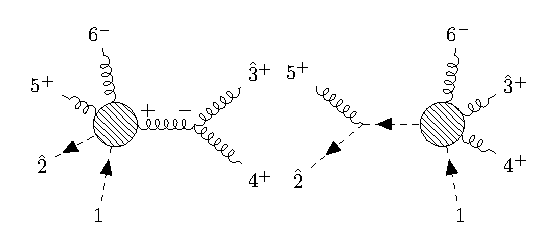
\includegraphics[width=0.6\textwidth]{6pt.eps}
    \end{figure}
    \vspace{-1em}
    \begin{align*}
    A_1&=\frac{(-1)\asqu{\hat{2}6}\asqu{16}}{\mdavg{25}{56}\!\avg{61}\!\mdavg{\hat{2}\hat{I}}{\hat{I}1}}\times\frac{1}{s_{34}}\times\frac{[\hat{3}4]^3}{[4\hat{I}][\hat{I}\hat{3}]}\notag\\
    &=\frac{\asqu{26}\avg{16}}{\mdavg{25}{56}\!\mdavg{\hat{2}\hat{I}}{\hat{I}1}}\times\frac{1}{s_{34}}\times\frac{[34]^3}{[4\hat{I}][\hat{I}3]}\notag\\
    &=\frac{\asqu{26}\avg{16}\bcancel{[34]^3}\bcancel{\avg{42}}}{\mdavg{25}{56}\!\mdavg{41}{32}\!\avg{43}\bcancel{[43][43][34]}\bcancel{\avg{24}}}\notag\\
    &=\frac{\asqu{26}\!\asqu{16}}{\textcolor{blue}{\mdavg{23}{34}\!\avg{41}}\!\textcolor{red}{\mdavg{25}{56}\!\avg{61}}}
    \end{align*}
\end{frame}
\begin{frame}
    \begin{itemize}
        \item Compact formula for general case
        \begin{equation*}
            A=\frac{\asqu{2\textcolor{green}{a}}\!\asqu{1\textcolor{green}{a}}}{\underbrace{\avg{2\textcolor{blue}{\star}}\cdots \avg{\textcolor{blue}{\star}1}}_{SU(N_1)}\underbrace{\avg{2\textcolor{red}{\ast} }\cdots \avg{\textcolor{red}{\ast} 1}}_{SU(N_2)}}
        \end{equation*} 
        \begin{minipage}{0.7\textwidth}
            \raggedright  % 或者 \centering 或 \raggedleft
            \textcolor{green}{Green:} \,Particle with $-$ helicity\\
            \textcolor{blue}{Blue:}\, Particle belongs to the first gauge group\\
            \textcolor{red}{Red:}\, Particle belongs to the second gauge group\\
            $\star$: \,Order for gauge group 1\\
            $\ast$: \,Order for gauge group 2 
            \end{minipage}
       
    \end{itemize}
    \pause
    For example, if we want to compute $A[1^\Phi2^{\Phi^\dagger}5_1^+3_1^+4_1^-7_2^+6_2^+8_2^+]$:
    \begin{equation*}
        A=\frac{\avg{2\textcolor{green}{4}}^2\avg{1\textcolor{green}{4}}^2}{\textcolor{blue}{\mdavg{25}{53}\mdavg{34}{41}}\textcolor{red}{\mdavg{27}{76}\mdavg{68}{81}}}
    \end{equation*}
    If you use Feynman diagrams, it may take sevral days to accomplish the computation.
\end{frame}
\section{Some problems and extends}
\begin{frame}
    \frametitle{How about NMHV?}
    First, let us review the NMHV amplitudes for gluon scattering.

    Still we begin with the simplest case -- \textbf{Split-helicity} NMHV like \mbox{\( A_6[1^-\, 2^-\, 3^-\, 4^+\, 5^+\, 6^+] \)}.%
    
    Here we choose $[1,2\rangle$ shift
\vspace{-1em}
\begin{figure}
    \centering
    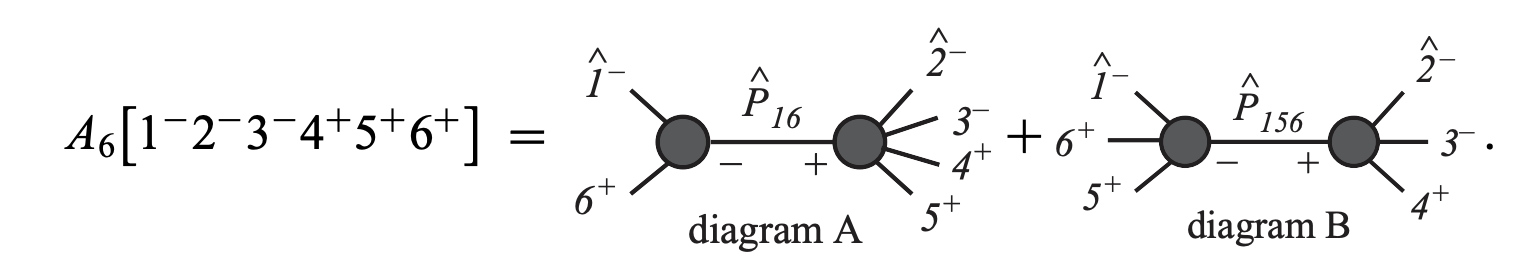
\includegraphics[width=1\textwidth]{6ptNMHV.png}
\end{figure}
\pause
\begin{itemize}
    \item Diagram B includes a propagator $1/P_{156}^2$, so there is a 3-particle pole $P_{156}^2=0$. But by inspecting the external order,
    it seems that there's no difference between $(-++)$ channel 561 and 345. We should expect the amplitude to have a pole also at 
    $P_{345}^2=0$. 
    \begin{equation*}
        \text{diagram A}=\frac{\avg{\hat{1}\hat{P}_{16}}^3}{\avg{\hat{P}_{16}6}\avg{6\hat{1}}}\times\frac{1}{P_{16}^2}\times\frac{\avg{\hat{2}3}^3}{\mdavg{34}{45}\!\mdavg{5\hat{P}_{16}}{\hat{P}_{16}2}}
    \end{equation*}
\end{itemize}
\end{frame}

\begin{frame}
    \begin{itemize}
    \item[] $$\cbrak{\hat{2} \hat{P}_{16}}{\hat{P}_{16} 3} = \avg{21}[\hat{1}3] + \avg{\hat{2}6}[63]$$
    It follows from $\hat{P}_{16}^2=0$ that $z_{16}=-\frac{[16]}{[26]}$, so
    \[
\cbrak{\hat{2} \hat{P}_{16}}{\hat{P}_{16} 3}
= -\frac{[36]}{[26]}
\left( \avg{12}[12] + \avg{16}[16] + \avg{26}[26] \right)
= -\frac{[36]}{[26]} P_{126}^2
\]
\textcolor{red}{The 3-particle pole $P_{126}^2$ is encoded inside the BCFW channel !}
    \item Full expression 
    \begin{align*}
        A_6[1^-\,2^-\,3^-\,4^+\,5^+\,6^+] =&
        \frac{ \langle 3|1+2|6]^3}{P_{126}^2 [21][16] \langle 34 \rangle \langle 45 \rangle \langle 5|1+6|2]}\\
        &+\frac{ \langle 1|5+6|4]^3}{P_{156}^2 [23][34] \langle 56 \rangle \langle 61 \rangle \langle 5|1+6|2]}.
    \end{align*}
    The factor $\langle 5|1+6|2]$ does not correspond to a physical pole of the scattering amplitude: it is a \textbf{spurious pole}.
    %You will also note that there is a strange denominator-factor $\langle 5|1+6|2]$ in the result from each BCFW diagram. 
    %It is typical that BCFW packs the information of the amplitudes into compact
    %expressions, but the cost is the appearance of spurious poles; this means that in the BCFW
    %representation the locality of the underlying field theory is not manifest.
    %The spurious pole should cancel in the sum of the two BCFW diagrams.

    There has been interesting paper investigating how to systematically cancel the spurious poles,
    like "A. Hodges, JHEP 1305, 35 (2013) [arXiv:0905.1473 [hep-th]]." 
    \end{itemize}
\end{frame}

\begin{frame}
    \begin{itemize}
        \item We utilize the $[1,2\rangle$ shift before, what happens if we change to $[2,1\rangle$ shift?
    \end{itemize}
    \begin{figure}
            \centering
            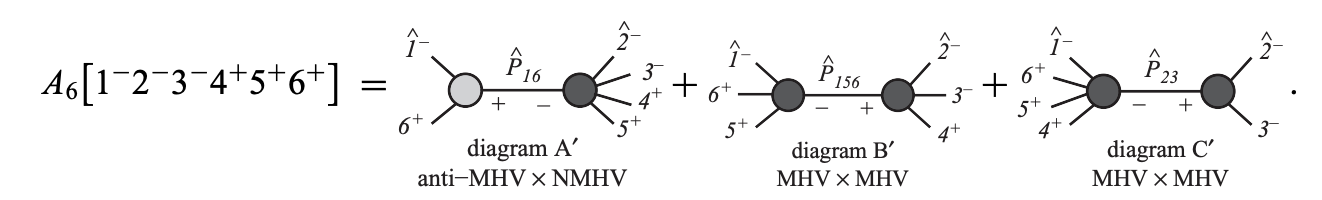
\includegraphics[width=1\textwidth]{6ptNMHV2.png}
        \end{figure}
    \begin{itemize}
        \item[] diagram A' = $\mathrm{anti\text{-}MHV} \times \mathrm{NMHV}$, as opposed to diagram A = $\mathrm{MHV}\times \mathrm{MHV}$. 
        \vspace{1em}

        \textcolor{red}{The equivalence between two different shift is related to powerful residue theorem} \textcolor{green}{(N. Arkani-Hamed, F. Cachazo, C. Cheung, and J. Kaplan, [arXiv:0907.5418 [hep-th]].)} \textcolor{red}{and Grassmannian.}
    \end{itemize}
\end{frame}
\begin{frame}
    \frametitle{CSW(Cachazo-Svrcek-Witten) expansion}
    We can also consider a shift that is implemented via a “holomorphic” square-spinor shift:
    \begin{equation*}
        \sket{\hat{i}}=\sket{i}+zc_i\sket{X},\qquad \aket{\hat{i}}=\aket{i}
    \end{equation*}
    Here $\sket{X}$ is an arbitrary reference spinor and the coefficients $c_i$ satisfy $\sum_{i=1}^{n} c_i \aket{i} = 0$.
    %Here we consider the situation where all $c_i\neq 0$, so that all momentum are shifted, called all-line shift.
    \begin{figure}
        \centering
        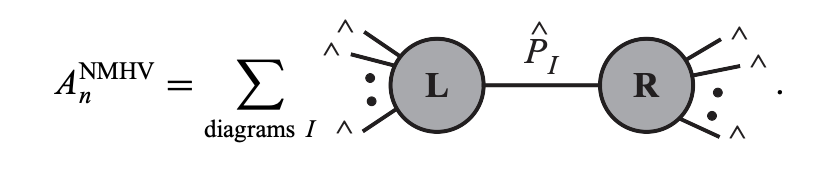
\includegraphics[width=0.7\textwidth]{NMHV.png}
    \end{figure}
    There are two possibilities: $\mathrm{anti\text{-}MHV_3}(=0)\times \mathrm{NMHV}$ ~or~ $\mathrm{MHV}\times\mathrm{MHV}$.
\end{frame}

\begin{frame}
    For example, the 6pt split NMHV amplitude
    \begin{figure}
        \centering
        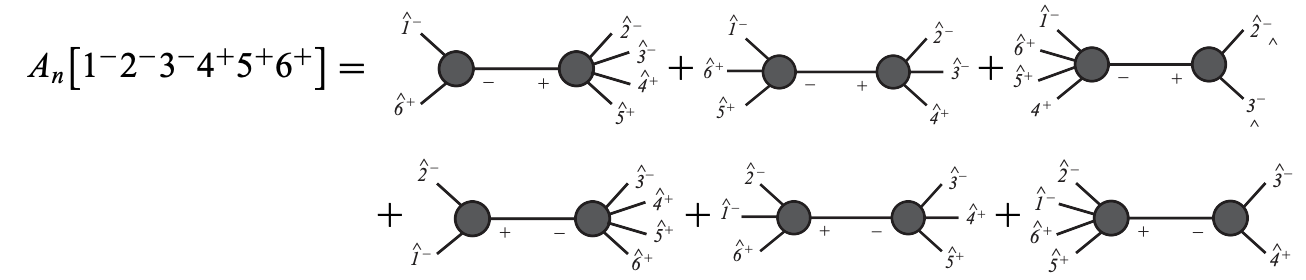
\includegraphics[width=1\textwidth]{6ptSpNMHV.png}
    \end{figure}

    \begin{minipage}{0.33\textwidth}
    \centering
    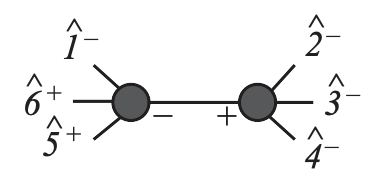
\includegraphics[width=1\textwidth]{exNMHV.png}
\end{minipage}
\hfill
\begin{minipage}{0.66\textwidth}
    \centering
    \[
    = \frac{\avg{1\hat{P}_I}^4}{\avg{1\hat{P}_I} \avg{\hat{P}_I 5} \avg{56} \avg{61}}
    \frac{1}{P_{156}^2}
    \frac{\avg{23}^4}{\avg{23} \avg{34} \avg{4\hat{P}_I} \avg{\hat{P}_I 2}} \,.
    \]
\end{minipage}
\pause

We can write 
\begin{equation*}
    \aket{\hat{P}_I}\frac{[\hat{P}_IX]}{[\hat{P}_IX]}=\hat{P}_I\sket{X}\frac{1}{[\hat{P}_IX]}=P_I\sket{X}\frac{1}{[\hat{P}_IX]}
\end{equation*}
\end{frame}
\begin{frame}
    We can use the prescription
    \begin{equation*}
        \aket{\hat{P}_I}\rightarrow P_I \sket{X}
    \end{equation*}
    \begin{minipage}{0.38\textwidth}
    \centering
    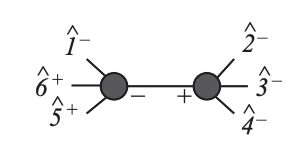
\includegraphics[width=\textwidth]{FinalNMHV.png}
\end{minipage}
\hfill
\begin{minipage}{0.62\textwidth}
    \centering
    \[
= \frac{\langle 1|P_{156}|X]^4}{\langle 1|P_{156}|X] \langle 5|P_{156}|X] \langle 56\rangle \langle 61\rangle}
\cdot \frac{1}{P_{156}^2}
\cdot \frac{\langle 23\rangle^4}{\langle 23\rangle \langle 34\rangle \langle 4|P_{156}|X] \langle 2|P_{156}|X]} \,.
\]

\end{minipage}

\end{frame}



\section{Summary}
\begin{frame}
    \frametitle{Summary}
    \begin{itemize}
        \item Introduce the on-shell method, including BCFW recursion relation, spinor-helicity formalism, etc.
        \item Introduce a (de)constructed gauge theory model, which is an effective field theory for 5 dimension gauge theory.
        \item Much of the scattering amplitudes in this model can be recursively computed by BCFW, and some compact formulas are offered.
    \end{itemize}
\end{frame}
\begin{frame} 
    \centering
    \Huge Thanks for your attention!
\end{frame} 
\appendix
\begin{frame}{Spinor-Helicity Formalism}
    \hypertarget{helicity}{}
\begin{block}{Helicity}
\textbf{\hyperlink{conv}{Helicity}} is defined as the projection of a particle's spin vector $\vec{S}$ onto the direction of its momentum $\vec{p}$:
\[
h = \frac{\vec{S} \cdot \vec{p}}{|\vec{p}|}
\]
\end{block}
\pause
% 文本说明(点击1出现)
\only<1->{
S-matrix is a function of momentum $p_i$ and helicity $h_i$
}

\vspace{0.8em}

% TikZ 图(点击1显示公式,点击2后补图形)
\begin{center}
\tikzset{every picture/.style={line width=0.75pt}}        
\begin{tikzpicture}[x=0.75pt,y=0.75pt,yscale=-1,xscale=1]

  % 点击1:显示公式
  \only<1>{
    \draw (260.25,137.9) node [anchor=north west][inner sep=0.75pt] 
          {$\mathcal{M}( p_{i} ,h_{i})$};
  }

  % 点击2及后:公式 + 圈箭头
  \only<2->{
    \draw (260.25,137.9) node [anchor=north west][inner sep=0.75pt] 
          {$\mathcal{M}( p_{i} ,\textcolor{red}{h_{i}})$};

    % 圆圈
    \draw  [color=red, draw opacity=1] 
      (302.8,146.93) .. controls (302.81,142.78) and (306.18,139.44) .. (310.32,139.45)
      .. controls (314.47,139.46) and (317.81,142.83) .. (317.8,146.97)
      .. controls (317.79,151.11) and (314.42,154.46) .. (310.28,154.45)
      .. controls (306.14,154.44) and (302.79,151.07) .. (302.8,146.93) -- cycle;

    % 箭头
    \draw [color=red, draw opacity=1] 
      (310.28,154.45) -- (296.03,178.04);
    \draw [shift={(295,179.75)}, rotate=301.13, color=red, draw opacity=1][line width=0.75pt] 
      (10.93,-3.29) .. controls (6.95,-1.4) and (3.31,-0.3) .. (0,0)
      .. controls (3.31,0.3) and (6.95,1.4) .. (10.93,3.29);

    % 注释文字
    \draw (173.25,181) node [anchor=north west][inner sep=0.75pt]  
      [font=\small,color=red,opacity=1] [align=left] 
      {How can we catch the information of helicity?};
  }

\end{tikzpicture}
\end{center}

% 点击3:Massless Case(用 uncover 保持排版稳定)
\uncover<3->{
\vspace{-1em}
\textbf{Massless Case:}
\begin{itemize}
  \item Momenta in spinor form:
    \[
      p_{\mu}\sigma^{\mu} = p_{\alpha\dot{\alpha}} = p_\alpha \tilde{p}_{\dot{\alpha}} = \aket{p}[p|
    \]
\end{itemize}
}

\end{frame}


\begin{frame}
    \frametitle{Large z behavior}
    In the BCFW formula, the boundary term $B_n$ affects a lot
    \begin{equation*}
        A_n=-\sum_{z_I}\mathrm{Res}|_{z=z_I}\frac{\hat{A}_n(z)}{z}+B_n,
    \end{equation*}
    In most applications. one assumes or much better, proves $B_n=0$. This is often justified by declaring a stronger condition
    \begin{equation*}
        \textcolor{red}{\hat{A}_n(z)\rightarrow 0 \quad \text{for} \quad z\rightarrow \infty} 
    \end{equation*}
    Here I show the large z behavior for gluon scattering 
    \begin{center}
        \begin{tabular}{lrc}
            \toprule
            $[i\, \textbackslash \, j\rangle $ & $+$ & $-$ \\
            \midrule
            $+$ & $1/z$ & $z^3$ \\
            $-$ & $1/z$ & $1/z$ \\
            \bottomrule
          \end{tabular}
    \end{center}
\end{frame}

\begin{frame}
        \textbf{On-shell 3-point for real momentum}

    Because of the constrain from momentum conservation and on-shell condition
    \begin{equation*}
        p_1=\kappa p_3, \qquad p_2=(1-\kappa)p_3 \quad(\text{Collinear})
    \end{equation*}
    All of the contribution 
    \begin{equation*}
        (p_1\cdot p_2),\quad (p_1\cdot p_3),\quad(p_2\cdot p_3)\quad =0  
    \end{equation*}
    In terms of Spinor- Helicity variable, we have 
    \begin{equation*}
        2p_1\cdot p_2=\avg{12}[21]=0\, \longrightarrow \,\avg{12}=[21]^*=0
    \end{equation*}
    \textcolor{red}{We can not obtain any thing nontrival from 3-point!}
    
    Of coure, you can introduce non-minimal interaction
    \begin{equation*}
        \mathcal{L}_3 \ni \frac{1}{\Lambda^2}\bar{\Psi}\slashed{D}(\Box \Psi)
    \end{equation*}
    but it still equals to 0 under the on-shell condition.
\end{frame}


\begin{frame}
    \frametitle{ On-shell 3-point can be completely determined}
    For the complex momentum, we have 
    \begin{equation*}
        \aket{1}\propto \aket{2}\propto \aket{3} \qquad or \qquad \sket{1}\propto \sket{2}\propto \sket{3}
    \end{equation*}
    \[
    \boxed{
    \begin{aligned}
        A_3^{h_1h_2h_3} &= c\avg{12}^{h_3-h_1-h_2}\avg{31}^{h_2-h_1-h_3}\avg{23}^{h_1-h_2-h_3}
        \quad & h_1+h_2+h_3 < 0 \\[0.5em]
        A_3^{h_1h_2h_3} &= c' [12]^{h_1+h_2-h_3}[23]^{h_2+h_3-h_1}[31]^{h_3+h_1-h_2}
        \quad & h_1+h_2+h_3 > 0
    \end{aligned}
        }
    \]

    \textbf{\textcolor{red}{$\star$\,All massless on-shell 3-point ampltides are completely determined by little group scaling!}}
    
    \textbf{Example}: 3-gluon amplitude\\
    \begin{equation*}
        A_3(g_1^-,g_2^-,g_3^+)=g\frac{\avg{12}^3}{\avg{23}\!\avg{31}}
    \end{equation*}
\end{frame}

\begin{frame}
    \frametitle{Scattering Amplitudes from BCFW}
    For simplicity, we start from the two-site gauge theory with gauge fields $V_1$, $V_2$ and scalar fields $\Phi$, $\Phi^\dagger$.
    \begin{equation*}
        \mathcal{L}=-\frac{1}{2}\mathrm{Tr}(F_1)^2-\frac{1}{2}\mathrm{Tr}(F_2)^2+\mathrm{Tr}[(D_\mu\Phi)^\dagger(D^\mu\Phi)],
    \end{equation*}
We only foucus on the following amplitudes:
\begin{equation*}
    \textcolor{red}{nV_1,\qquad nV_2,\qquad\Phi^\dagger nV_1 \Phi,\qquad \Phi nV_2 \Phi^\dagger,\qquad \Phi^\dagger \Phi\Phi^\dagger \Phi}
\end{equation*}
here n can be any positive integer.
\end{frame}

\begin{frame}
    More specifically, it helps us to prove P. T. formula

\begin{center}
\tikzset{every picture/.style={line width=0.75pt}} %set default line width to 0.75pt        

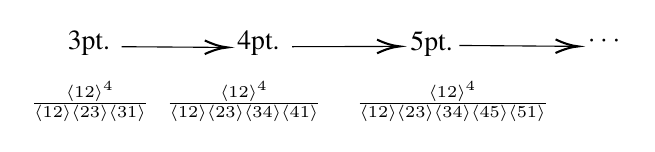
\begin{tikzpicture}[x=0.75pt,y=0.75pt,yscale=-1,xscale=1]
%uncomment if require: \path (0,300); %set diagram left start at 0, and has height of 300

%Straight Lines [id:da4236245229594603] 
\draw    (259,91.9) -- (308,92.24) ;
\draw [shift={(310,92.25)}, rotate = 180.39] [color={rgb, 255:red, 0; green, 0; blue, 0 }  ][line width=0.75]    (10.93,-3.29) .. controls (6.95,-1.4) and (3.31,-0.3) .. (0,0) .. controls (3.31,0.3) and (6.95,1.4) .. (10.93,3.29)   ;
%Straight Lines [id:da22408043084764206] 
\draw    (341.2,91.9) -- (391,91.76) ;
\draw [shift={(393,91.75)}, rotate = 179.83] [color={rgb, 255:red, 0; green, 0; blue, 0 }  ][line width=0.75]    (10.93,-3.29) .. controls (6.95,-1.4) and (3.31,-0.3) .. (0,0) .. controls (3.31,0.3) and (6.95,1.4) .. (10.93,3.29)   ;
%Straight Lines [id:da5239716133788715] 
\draw    (421.7,91.3) -- (477,91.73) ;
\draw [shift={(479,91.75)}, rotate = 180.45] [color={rgb, 255:red, 0; green, 0; blue, 0 }  ][line width=0.75]    (10.93,-3.29) .. controls (6.95,-1.4) and (3.31,-0.3) .. (0,0) .. controls (3.31,0.3) and (6.95,1.4) .. (10.93,3.29)   ;

% Text Node
\draw (231.8,83.1) node [anchor=north west][inner sep=0.75pt]   [align=left] {{\fontfamily{ptm}\selectfont 3pt.}};
% Text Node
\draw (313.5,83) node [anchor=north west][inner sep=0.75pt]   [align=left] {{\fontfamily{ptm}\selectfont 4pt.}};
% Text Node
\draw (396.9,83.5) node [anchor=north west][inner sep=0.75pt]   [align=left] {{\fontfamily{ptm}\selectfont 5pt.}};
% Text Node
\draw (482.4,85.2) node [anchor=north west][inner sep=0.75pt]    {$\cdots $};
% Text Node
\draw (214,107.4) node [anchor=north west][inner sep=0.75pt]  [font=\small]  {$\frac{\langle 12\rangle ^{4}}{\langle12\rangle\langle 23\rangle \langle 31\rangle }$};
% Text Node
\draw (279.25,107.4) node [anchor=north west][inner sep=0.75pt]  [font=\small]  {$\frac{\langle 12\rangle ^{4}}{\langle 12\rangle \langle 23\rangle \langle 34\rangle \langle 41\rangle }$};
% Text Node
\draw (370.75,107.4) node [anchor=north west][inner sep=0.75pt]  [font=\small]  {$\frac{\langle 12\rangle ^{4}}{\langle 12\rangle \langle 23\rangle \langle 34\rangle \langle 45\rangle \langle 51\rangle }$};


\end{tikzpicture}
\end{center}  
 
\vspace{-2em}
\pause
\begin{equation*}
    \boxed{\Rightarrow:\quad A[1^+\cdots ~i^-(i+1)^+\cdots~j^-(j+1)^+\cdots n^+]=\frac{\avg{ij}^4}{\avg{12}\!\avg{23}\cdots\avg{n1}}}
\end{equation*}

\vspace*{2em}
\textcolor{red}{$\bigstar$ \Large This is the power of BCFW recursion relation.}
\end{frame}

\end{document}